\documentclass[hyperref={pdfpagelabels=false}]{beamer}
\setbeamertemplate{caption}[numbered]
\usepackage[utf8]{inputenc}
\usepackage[spanish]{babel}
\spanishdecimal{.}


\input{tecbeamer.tex}

\title{\textbf{Validación experimental de controladores para multi-agentes tipo Quad-Rotor}}  
\author[]{\textbf{Alumno:} Ing. Julio Cesar Rodríguez Cervantes \\
\textbf{Asesor:} Dr. Alejandro Enrique Dzul López}
\title[Ing. Julio Cesar Rodríguez Cervantes]{\textbf{Validación experimental de controladores para multi-agentes tipo Quad-Rotor}} 
\institute{\textbf{TecNM Campus La Laguna}} 
\date{22 de febrero 2022}

\begin{document}

\maketitleandtoc
\section{Motivaci\'on}
\begin{frame}{Motivaci\'on}\justifying
%The Scientific Papers of James Clerk Maxwell\footfullcite{maxwell1890scientific}.
%Los vehículos aéreos no tripulados (UAVs por sus siglas en inglés) han tenido últimamente un auge importante debido a la gran variedad de aplicaciones en distintas áreas, tales como salud, vigilancia, transporte, espectáculos, mapeos de áreas, reconocimiento y localización de objetos. En cuanto a la investigación estos han sido de interés debió a su tamaño, a su modo de vuelo y su reducido costo, en comparación a otro tipo de vehículos aéreos no tripulados.
%Otra área de estudio que ha tomado relevancia es la cooperación de múltiples vehículos, para la coordinación de movimiento, se busca diseñar leyes de control de formación que permitan que un grupo de robots mantengan un patrón geométrico deseado, para que estos ejecuten una tarea, en la figura \ref{TM} se muestran distintos tipos de tareas aplicados con multiagentes.
\begin{figure}[h]

\centering  
\subfigure[Reconocimiento]{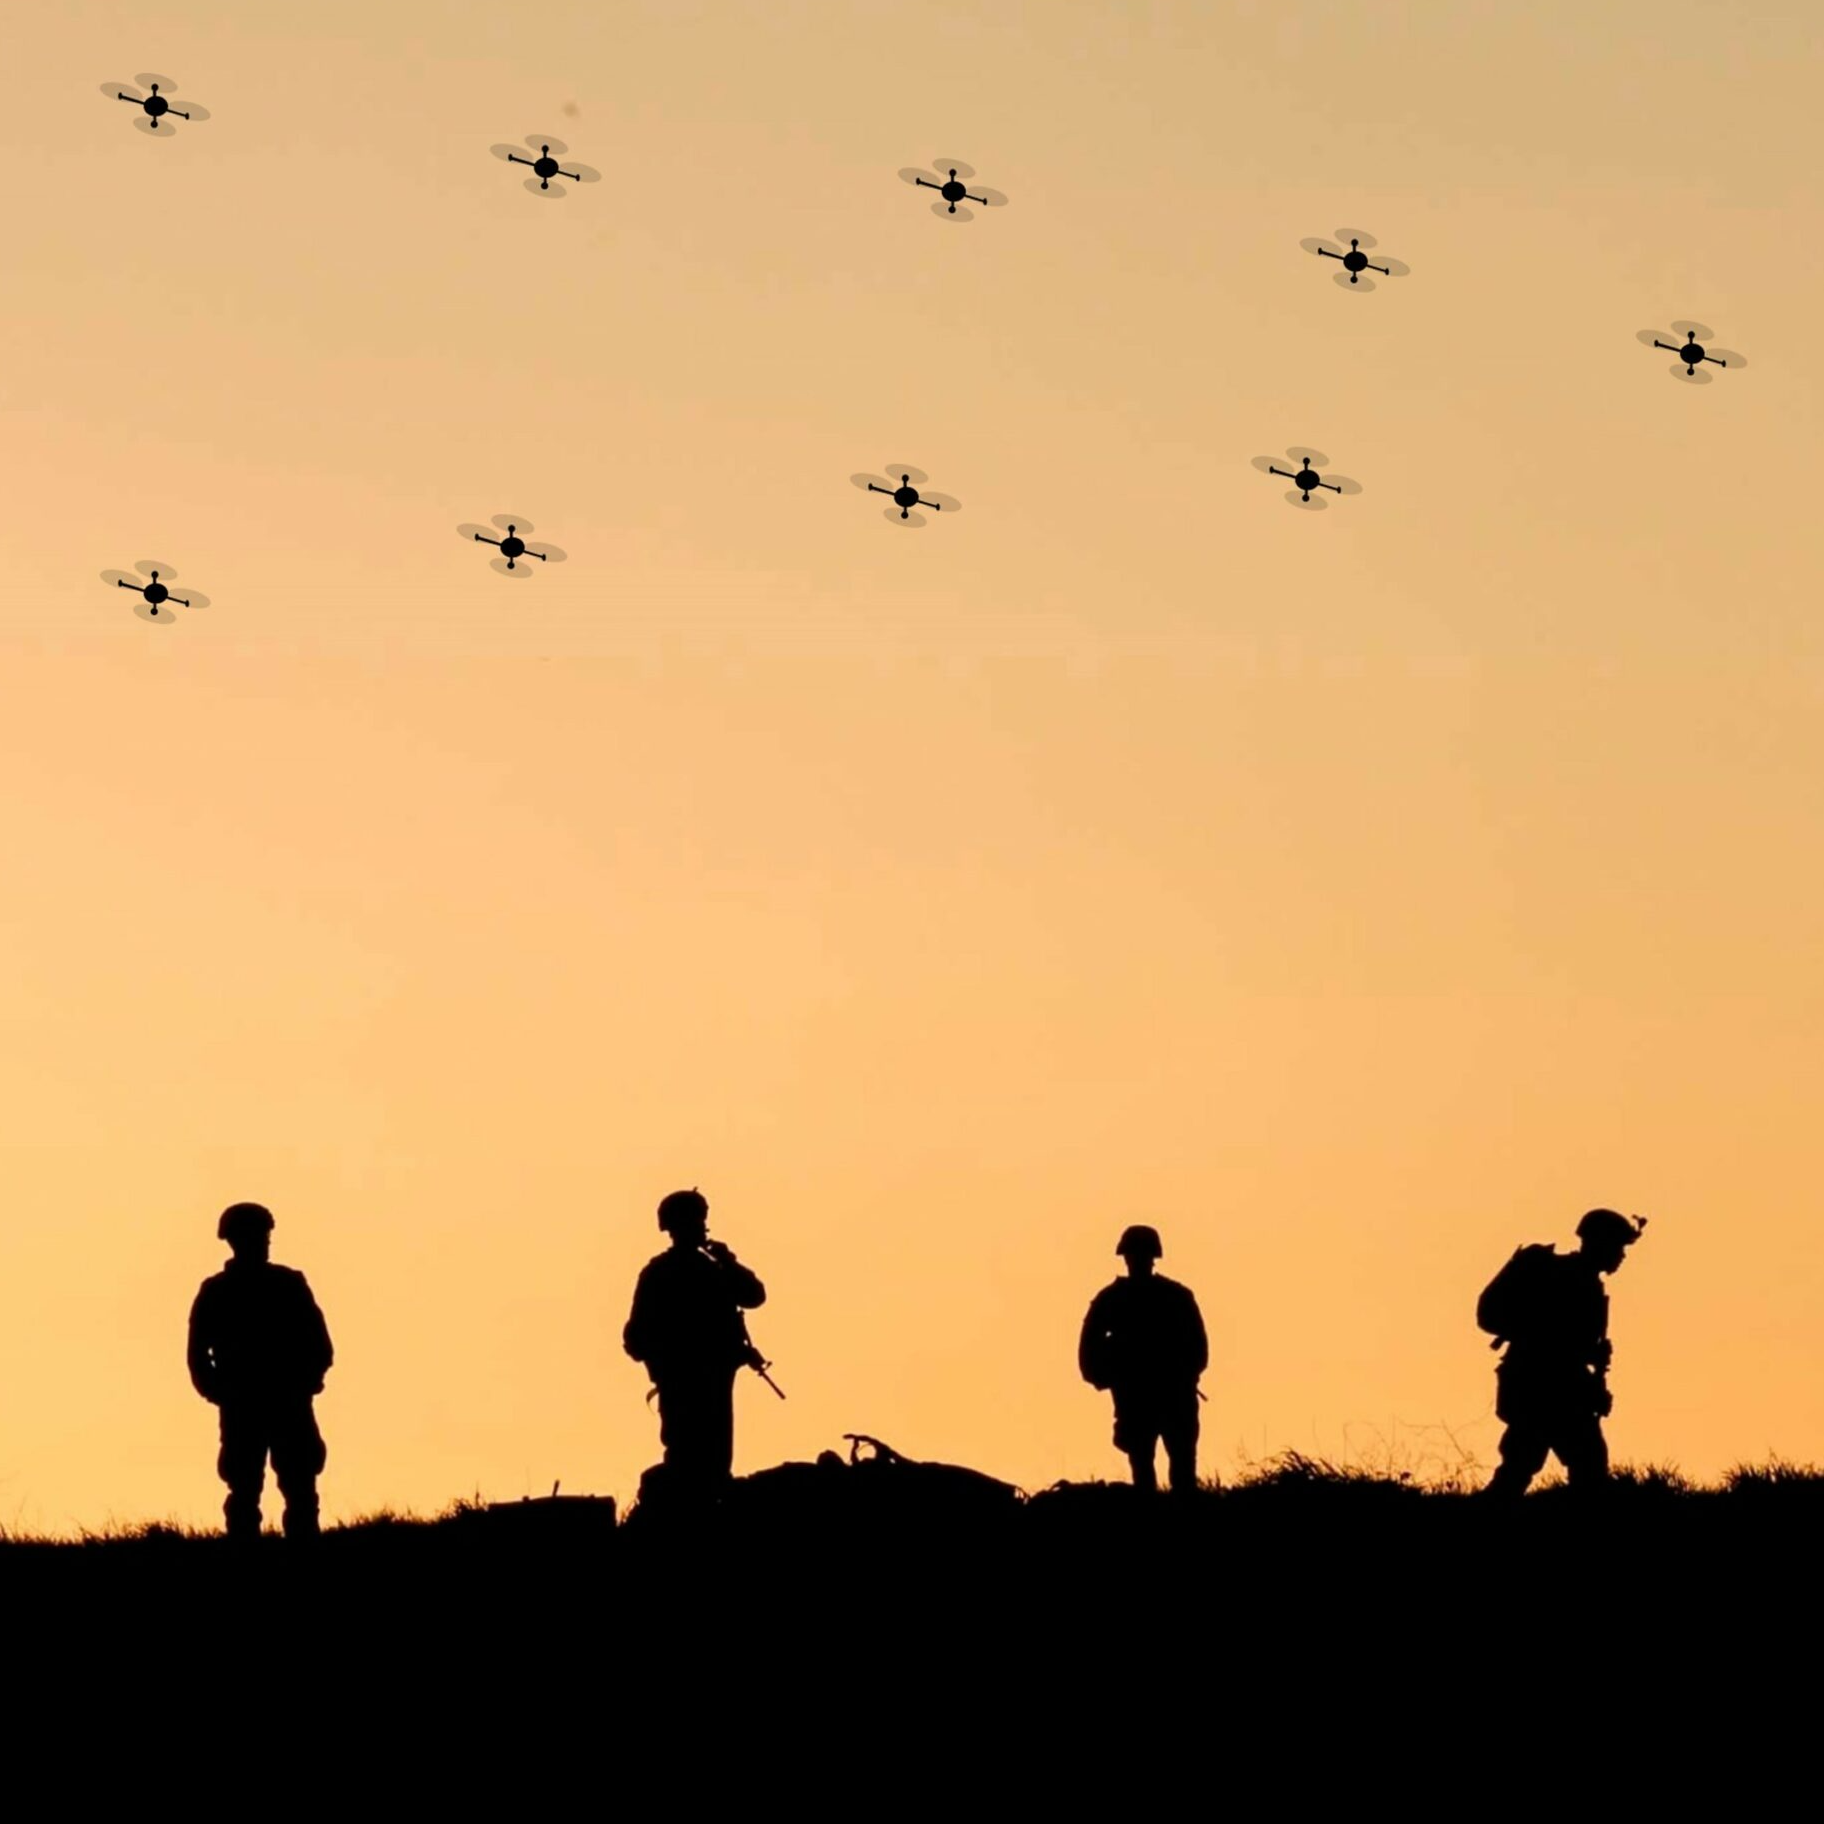
\includegraphics[width=0.2\linewidth]{Figures/combate.png}}
\subfigure[Mapeo de áreas]{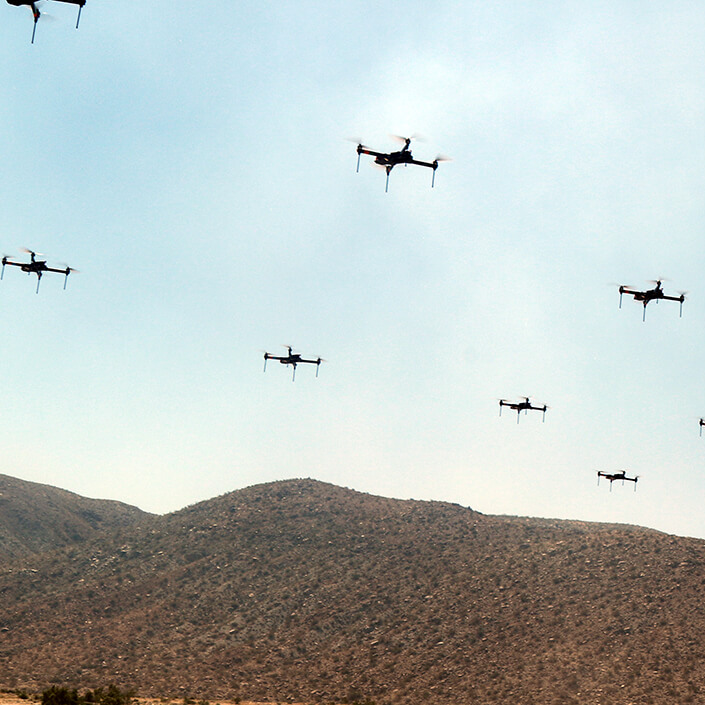
\includegraphics[width=0.2\linewidth]{Figures/Reconocimiento.png}}
\subfigure[Transporte]{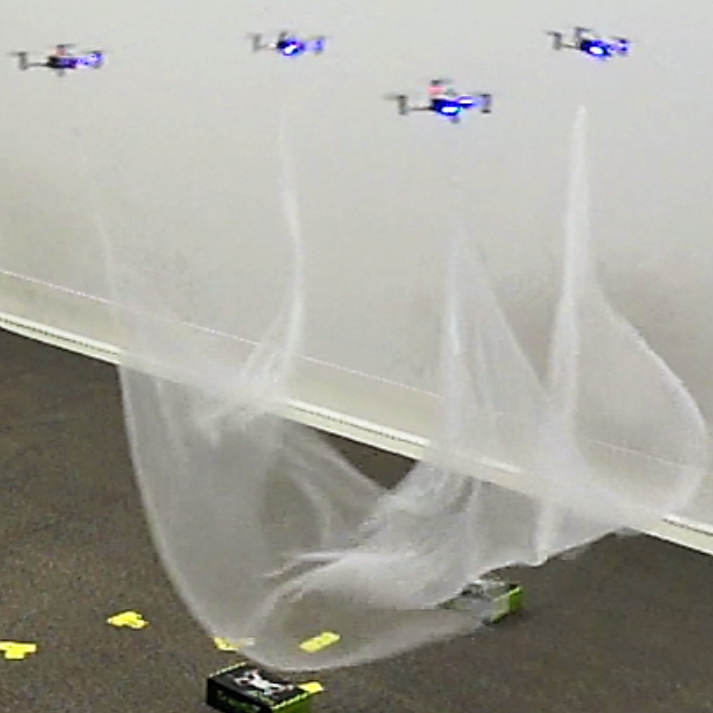
\includegraphics[width=0.2\linewidth]{Figures/Transporte.png}}
\subfigure[Espectáculo]{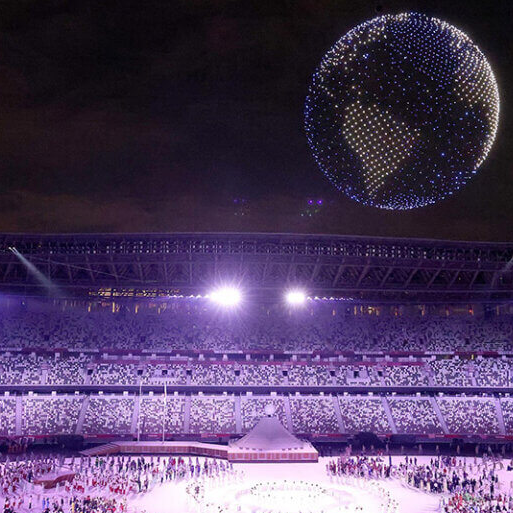
\includegraphics[width=0.2\linewidth]{Figures/world.png}}
\caption{Tareas con Multiagentes.}\label{TM}
\end{figure}


%\begin{block}{Move with me}
%    Chant with me.\\
%    And if you're good, I'll take you home with me
%\end{block}
\end{frame}



\section{Objetivos} 
\begin{frame}{Objetivos} 
\begin{itemize}
\item Estudio de los controladores virtuales aplicados para agentes de los trabajos \footfullcite{inproceedings} \footfullcite{rios2018continuous}
\item Avances experimentales.
\end{itemize}
\end{frame}

\section{Planteamiento del problema} 
\begin{frame}{Modelado de un Quad-Rotor} 
Considere un grupo de dos Quad-Rotor.
La dinámica simplificada de cada uno de ellos (ver Figura \ref{Figquad}, y para detalles de modelado, ver \footfullcite{carrillo2013quad}), está dada por: 
\begin{subequations}
  \begin{align}
	\dot{\xi}_1  &= \xi_2 ,\\
	\dot{\xi_2}  &=g_{\xi}(\eta_1)u_m-G,\\
	\dot{\eta_1} &= \eta_2,\\
	\dot{\eta_2} &= J\tau+\Xi w(\eta_2)+d_{\eta}. 
   \end{align}\label{eq: Dinamica del quad}
\end{subequations}

donde $\xi_1 := [x,~y,~z]^T~ \in \mathbb{R}^3$, $\xi_2 := [\dot{x},~\dot{y},~\dot{z}]^T~ \in \mathbb{R}^3$, $\eta_1 := [\phi,~\theta,~\psi]^T~ \in \mathbb{R}^3$, $\eta_2 := [\dot{\phi},~\dot{\theta},~\dot{\psi}]^T~ \in \mathbb{R}^3$, $d_{\eta} := \diago[d_{\phi},~d_{\theta},~d_{\psi}]^T~ \in \mathbb{R}^3$.
\end{frame}



\begin{frame}{Modelado de un Quad-Rotor} 
 Los términos $G := [0,~0,~g]^T~\mathbb{R}^3$, $J := \diago[J_x^{-1},~J_y^{-1},~J_z^{-1}]^T~\mathbb{R}^{3\times 3}$ y   $\tau := [\tau_{\phi},~\tau_{\theta},~\tau_{\psi}]^T~\mathbb{R}^3$ son el vector de gravedad, la matriz de inercia y el vector de momento angular. El t\'ermino $u_m :=u_z/m$. La matriz $\Xi := \diago {[b_{\phi},~b_{\theta},~b_{\psi}]}~ \in \mathbb{R}^{3 \times 3}$, est\'a dada por los coeficientes de inercia  $b\phi := (J_y -J_z)/J_x$, $b\theta := (J_z -J_x)/J_y$ y $b\psi := (J_x - J_y)/J_z$. Las funciones $g_{\xi}(\eta_1):=[\cos\phi \sen\theta \cos\psi + \sen\phi \sen\psi,~ \cos\phi \sen\theta \sen\psi + \sen\phi \cos\psi,~ \cos\phi \cos\theta ]^T $ y $w_{\eta}(\eta_2):=[\dot{\theta}\dot{\psi},~ \dot{\phi}\dot{\psi},~ \dot{\psi}\dot{\theta} ]^T$, respectivamente.
\end{frame}


\begin{frame}{Modelado de un Quad-Rotor} 
\begin{figure}[H]
\centering
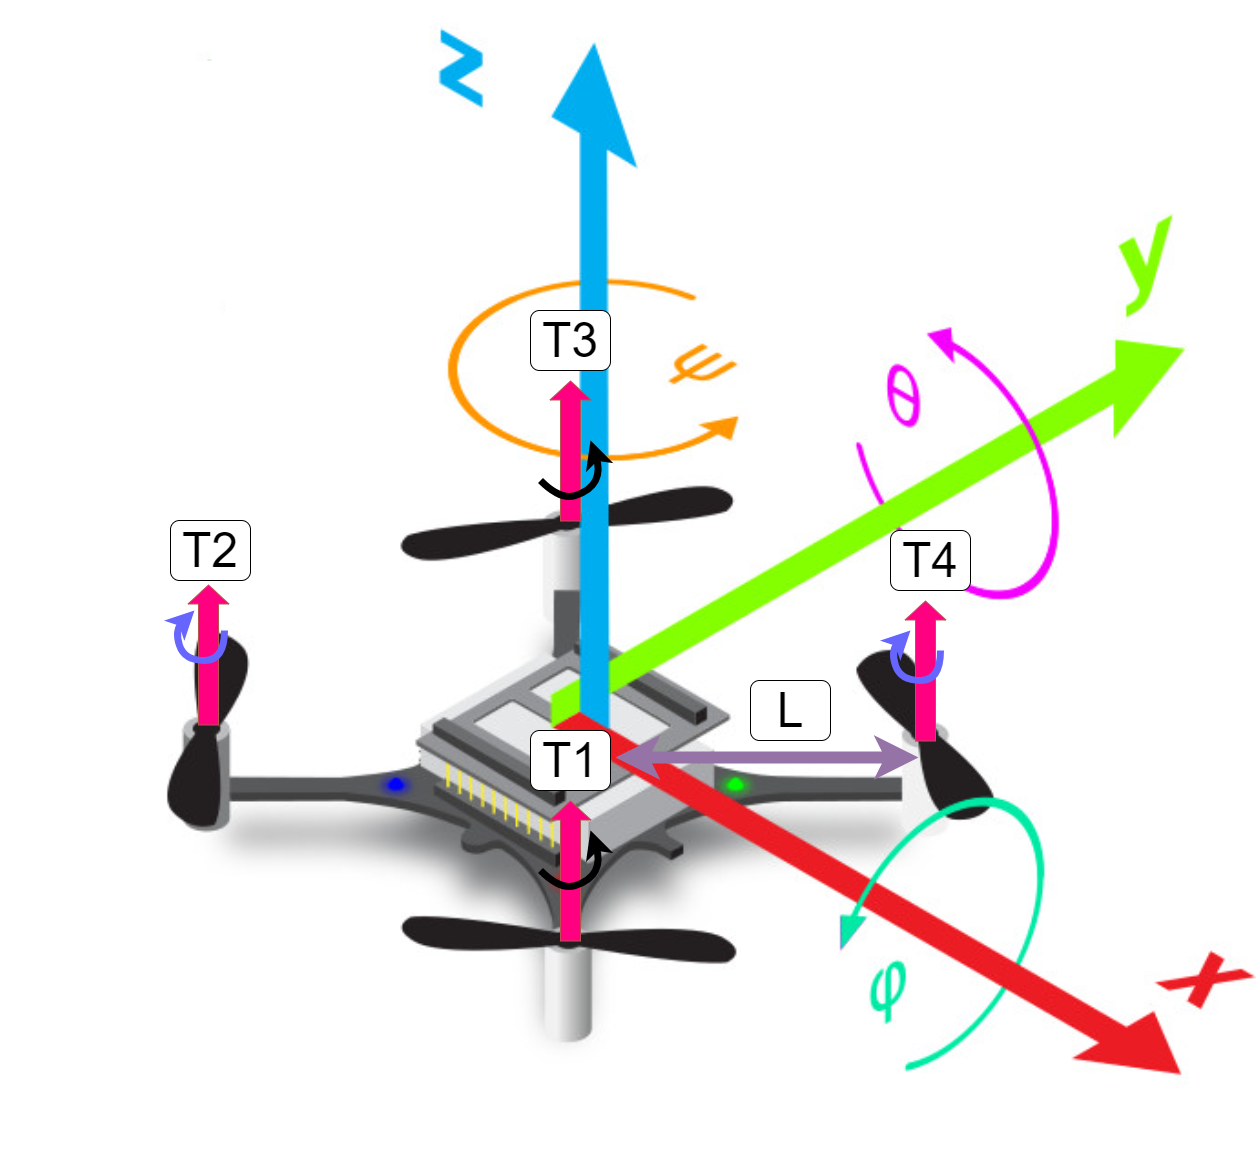
\includegraphics[scale=.11]{Figures/crazy.png}
\caption{Representación esquemática del Quad-Rotor}\label{Figquad}
\end{figure}
\end{frame}

\begin{frame}{Dinámica del error del Quad-Rotor Líder} 
Sea la dinámica del error del Quad-Rotor líder de la siguiente forma:
\begin{subequations}
  \begin{align}
	\dot{e}_{\xi_L}            &= \dot{\xi}_{1_L}  - \dot{\xi}_{1_L}= \varepsilon_{\xi_L}, \\ 
	\dot{\varepsilon}_{\xi_L}  &= \dot{\xi}_{2_L}  - \ddot{\xi}_{d} =g_{\xi_{L}}(\eta_{1_L})u_{m_L}-G-\ddot{\xi_{d}},\\ 
	\dot{e}_{\eta_L}           &= \dot{\eta}_{1_L} - \dot{\eta}_{d},\\ \label{eq:Dinamica del error Lider c}
	\dot{\varepsilon}_{\eta_L} &= \dot{\eta}_{2_L} - \ddot{\eta}_d = J\tau+\Xi w_{\eta_2}(\eta_{2_L})+d_{\eta_L} -\ddot{\eta_d}.
  \end{align}\label{eq:Dinamica del error Lider}
\end{subequations}

\end{frame}

\begin{frame}{Cálculo de las señales de referencia del líder.} 
Se introduce un control virtual $\nu_L~ \in~\mathbb{R}^3 $ en (\ref{eq:Dinamica del error Lider}b) 
\begin{equation}
\dot{\varepsilon}_{\xi_L} = \nu_L + \omega(\eta_{1_L}) - G,
\end{equation}
donde
\begin{equation*}
    \omega(\eta_{1_L}) = u_{m_L}  g_{\xi_{_L}}(\eta_{1_L}) - G -\nu_L,
\end{equation*}
por lo tanto,
\begin{equation*}
    \nu_L =u_{m_L}  g_{\xi_{L}}(\eta_{d}) - G,
\end{equation*}
puede ser expresado como:
\begin{subequations}
  \begin{align}
\nu_{x_L} &= u_{m_L} (\cos{\phi_{\star_L}}\sen{\theta_{\star_L}}\cos{\psi_{d}} + \sen{\phi_{\star_L}}\sen{\psi_{d}}),\\
\nu_{y_L} &= u_{m_L}(\cos{\phi_{\star_L}}\sen{\theta_{\star_L}}\sen{\psi_{d}} - \sen{\phi_{\star_L}}\cos{\psi_{d}}),\\
\nu_{z_L} &= u_{m_L}(\cos{\phi_{\star_L}}\cos{\theta_{\star_L}})-g.
  \end{align}\label{eq:nulid}
\end{subequations}
\end{frame}


\begin{frame}{Cálculo de las señales de referencia del líder.} 
Despejando $\phi_{\star_L}$, $\theta_{\star_L}$ y $u_{m_L}$ de (\ref{eq:nulid}), se obtiene (\ref{eq:desl})
\begin{subequations}
  \begin{align}
    \phi_{\star_L} &= \arcsin{[u_{m_L}^{-1}(\nu_{x_L} \sen{\psi_{d_L}} - \nu_{y_L} \cos{\psi_{d_L} }]}, \\
    \theta_{\star_L} &= \arctan{[(\nu_{z_L} + g )^{-1}(\nu_{x_L} \cos{\psi_{d}} + \nu_{y_L} \sen{\psi_{d} }]}, \\
    u_{m_L} & = \sqrt{\nu_{x_L}^2+\nu_{y_L}^2+ (\nu_{z_L}+g)^2},
    \end{align}
  \label{eq:desl}
\end{subequations}
donde los controladores virtuales están representados por:
\begin{subequations}
  \begin{align}
    \nu_{x_L} &=k_{x_0}\Bar{e}_{x_L}+ k_{x_1}e_{x_L} + k_{x_3}\varepsilon_{x_L} + \ddot x_{d} ,\\
    \nu_{y_L} &=k_{y_0}\Bar{e}_{y_L}+ k_{y_1}e_{y_L} + k_{y_3}\varepsilon_{y_L}  + \ddot y_{d},\\
    \nu_{z_L} &= k_{z_0}\Bar{e}_{z_L}+ k_{z_1}e_{z_L} + k_{z_3}\varepsilon_{z_L} + \ddot z_{d} ,
    \end{align}
  \label{eq:cv2}
\end{subequations}
\end{frame}


\begin{frame}{Dinámica del error del Quad-Rotor l\'ider.} 
Sea la dinámica del error del Quad-Rotor seguidor de la siguiente forma:
\begin{subequations}
  \begin{align}
	\dot{e}_{\xi_S}            &= \dot{\xi}_{1_S}  - \dot{\xi}_{1_S}  = \varepsilon_{\xi_S},\\ 
	\dot{\varepsilon}_{\xi_S}  &= \dot{\xi}_{2_S}  - \dot{\xi}_{2_L}  = g_{\xi_{S}}(\eta_{1_S})u_{m_S}-G-\dot{\xi}_{2_L},\\ 
	\dot{e}_{\eta_S}           &= \dot{\eta}_{1_S} - \dot{\eta}_{1_S},\\ 
	\dot{\varepsilon}_{\eta_S} &= \dot{\eta}_{2_S} - \dot{\eta}_{2_L} = J\tau+\Xi w_{\eta_2}(\eta_{2_S})+d_{\eta_S} -\dot{\eta}_{2_L}.
  \end{align}\label{eq:Dinamica del error Seguidor}
\end{subequations}
Sustituyendo (\ref{eq: Dinamica del quad}b) del líder en (\ref{eq:Dinamica del error Seguidor}b) se tiene: 
\begin{subequations}
  \begin{align}
    \dot{\varepsilon}_{\xi_S}  &=  g_{\xi_{S}}(\eta_{1_S})u_{m_S}-G-(g_{\xi_{L}}(\eta_{1_L})u_{m_L}-G),\\ 
     &=  g_{\xi_{S}}(\eta_{1_S})u_{m_S}-g_{\xi_{L}}(\eta_{1_L})u_{m_L},\\ 
     &=  g_{\xi_{S}}(\eta_{1_S})u_{m_S}-g_{\xi_{L}}(\eta_{1_L})u_{m_L}.
  \end{align}\label{eq:diner}
\end{subequations}
\end{frame}

%---------------------------
\begin{frame}{Cálculo de las señales de referencia del seguidor.} 
Se introduce un control virtual $\nu_1~ \in~\mathbb{R}^3 $ en (\ref{eq:diner}) 
\begin{equation}
\dot{\varepsilon}_{\xi_S} = \nu_S + \omega(\eta_{1_S}),
\end{equation}
donde
\begin{equation*}
\begin{split}
    \omega(\eta_{1_S}) &= u_{m_S}  g_{\xi_{S}}(\eta_{1_S})- \gamma(\eta_{1_L},u_{m_L})-\nu_S,\\
    \gamma(\eta_{1_L}, u_{m_L}) &=u_{m_L}g_{\xi_{L}}(\eta_{1_L}),
\end{split}
\end{equation*}
por lo tanto,
\begin{equation*}
    \nu_S =u_{m_S}  g_{\xi_{S}}(\eta_{d_S})- \gamma(\eta_{1_L},u_{m_L}),
\end{equation*}
puede ser expresado como:
\begin{subequations}
  \begin{alignat}{2}
\nu_{x_S} &= u_{m_S} (\cos{\phi_{\star_S}}\sen{\theta_{\star_S}}\cos{\psi_{d_S}} + \sen{\phi_{\star_S}}\sen{\psi_{d_S}}) -\gamma_x,\\
\nu_{y_S} &= u_{m_S}(\cos{\phi_{\star_S}}\sen{\theta_{\star_S}}\sen{\psi_{d_S}} - \sen{\phi_{\star_S}}\cos{\psi_{d_S}}) -\gamma_y,\\
\nu_{z_S} &= u_{m_S}(\cos{\phi_{\star_S}}\cos{\theta_{\star_S}}) -\gamma_z,
  \end{alignat}\label{eq:nuseg}
\end{subequations}
\end{frame}


\begin{frame}{Cálculo de las señales de referencia del seguidor.} 
despejando $\phi_{\star_S}$, $\theta_{\star_S}$ y $u_{m_S}$ de (\ref{eq:nuseg}), se obtiene
\begin{subequations}
  \begin{alignat}{2}
    \phi_{\star_S} &= \arcsin{[u_{m_S}^{-1}((\nu_{x_S}+\gamma_x )\sen{\psi_{d_S}} - (\nu_{y_S}+\gamma_y) \cos{\psi_{d_S} }]}, \\
    \theta_{\star_S} &= \arctan{[(\nu_{z_S}+\gamma_z)^{-1}((\nu_{x_S}+\gamma_x) \cos{\psi_{d_S}} + (\nu_{y_S}+\gamma_y) \sen{\psi_{d_S} }]}, \\
    u_{m_S} & = \sqrt{(\nu_{x_S}+\gamma_x)^2+(\nu_{y_S}+\gamma_y)^2+ (\nu_{x_S}+\gamma_z)^2}, 
  \end{alignat}
  \label{eq:dess}
\end{subequations}

donde los controladores virtuales están representados por:
\begin{subequations}
  \begin{align}
    \nu_{x_S} &=k_{x_0}\Bar{e}_{x_S}+ k_{x_1}e_{x_S} + k_{x_3}\varepsilon_{x_S},\\
    \nu_{y_S} &=k_{y_0}\Bar{e}_{y_S}+ k_{y_1}e_{y_S} + k_{y_3}\varepsilon_{y_S},\\
    \nu_{z_S} &=k_{z_0}\Bar{e}_{z_S}+ k_{z_1}e_{z_S} + k_{z_3}\varepsilon_{z_S},
    \end{align}
  \label{eq:cv2}
\end{subequations}
\end{frame}


% Calculo de las senales de referencia partiendo del sistema linealizado.
%\begin{frame}{Cálculo de las señales de referencia del l\'ider partiendo del sistema linealizado.} 
%
%Se consideran los siguientes subsistemas de la dinámica de posición del Quad-Rotor para el análisis de las se\~nales de referencia del líder.
%\vspace{1em}
%
%\begin{center}
%	\textbf{Subsistema X}
%	\vspace{.1em}
%	
%	$\dot{x}_1 = x_2,$
%	\vspace{.1em}
%	
%	$\dot{x}_2 = f(x)+g(x)u_1,$
%	\vspace{.1em}
%	
%	$f(x)= 0,$
%	\vspace{.1em}
%	
%	$g(x)= \frac{\cos{\phi_L}\sin{\theta_L}\cos{\psi_L}+\sin{\phi_L}\sin{\psi_L}}{m},$
%\end{center}
%
%donde 
%\begin{center}
%	\vspace{.1em}
%	
%	$x_1 = x,$
%	\vspace{.1em}
%	
%	$x_2 = \dot{x},$
%	\vspace{.1em}
%
%	$u_1 = u_z.$
%\end{center}
%\end{frame}
%
%\begin{frame}{Cálculo de las señales de referencia del l\'ider partiendo del sistema linealizado.} 
%	
%\begin{center}
%	\textbf{Subsistema Y}
%	\vspace{.1em}
%	
%	$\dot{y}_1 = y_2,$
%	\vspace{.1em}
%	
%	$\dot{y}_2 = f(y)+g(y)u_1,$
%	\vspace{.1em}
%	
%	$f(y)= 0,$
%	\vspace{.1em}
%	
%	$g(y)= \frac{\cos{\phi_L}\sin{\theta_L}\sin{\psi_L}+\sin{\phi_L}\cos{\psi_L}}{m},$
%\end{center}
%
%donde 
%\begin{center}
%	\vspace{.1em}
%	
%	$y_1 = y,$
%	\vspace{.1em}
%	
%	$y_2 = \dot{y},$
%	\vspace{.1em}
%	
%	$u_1 = u_z.$
%\end{center}
%\end{frame}
%
%\begin{frame}{Cálculo de las señales de referencia del l\'ider partiendo del sistema linealizado.} 
%	
%	\begin{center}
%		\textbf{Subsistema Z}
%		\vspace{.1em}
%		
%		$\dot{z}_1 = z_2,$
%		\vspace{.1em}
%		
%		$\dot{z}_2 = f(z)+g(z)u_1,$
%		\vspace{.1em}
%		
%		$f(z)= -g,$
%		\vspace{.1em}
%		
%		$g(z)= \frac{\cos{\phi_L}\cos{\theta_L}}{m},$
%	\end{center}
%	
%	donde 
%	\begin{center}
%		\vspace{.1em}
%		
%		$y_1 = y,$
%		\vspace{.1em}
%		
%		$y_2 = \dot{y},$
%		\vspace{.1em}
%		
%		$u_1 = u_z.$
%	\end{center}
%\end{frame}

\begin{frame}{Cálculo de las señales de referencia del l\'ider linealizando el sistema.} 
	Partiendo de $\ddot{x_L}$, y linealizando.
\begin{equation}
	\ddot{x_L} = \frac{u_L \sen{\theta_L}}{m}.
\end{equation}

La dinámica del error esta dada por: 
\begin{equation}
	\begin{split}
		\varepsilon_{x_L} &= \ddot{x_L} - \ddot{x_d},\\
		&= \frac{u_L \sen{\theta_L}}{m} - \ddot{x_d}.
	\end{split}	
\end{equation}
\end{frame}


\begin{frame}{Cálculo de las señales de referencia del l\'ider linealizando el sistema.} 
Se introduce un control virtual $\nu_{x_L}$
	\begin{equation}
		\begin{split}
			\varepsilon_{x_L} &= \nu_{x_L} + \omega(\theta_L,u_L),\\
			\omega(\theta_L,u_L) &= \frac{u_L \sen{\theta_L}}{m} - \nu_{x_L},\\
			\nu_{x_L} &= \frac{u_L \sen{\theta_{\star_L}}}{m},
		\end{split}
	\end{equation}
despejando $\theta_{\star_L}$
\begin{equation}
	\begin{split}
		\sen{\theta_{\star_L}} &= \frac{m \nu_{x_L}}{u_L},\\
		\theta_{\star_L} &= \arcsen{\bigg(\frac{m \nu_{x_L}}{u_L}\bigg)},\\
	\end{split}
\end{equation}
\end{frame}

\begin{frame}{Cálculo de las señales de referencia del l\'ider linealizando el sistema.} 
	Partiendo de $\ddot{y_L}$, y linealizando el subsistema.
	\begin{equation}
		\ddot{y_L} = -\frac{u_L \sen{\phi_L}}{m}.
	\end{equation}
	
	La dinámica del error esta dada por: 
	\begin{equation}
		\begin{split}
			\varepsilon_{y_L} &= \ddot{y} - \ddot{y_d},\\
			&=-\frac{u_L \sen{\phi_L}}{m} - \ddot{y_d}.
		\end{split}	
	\end{equation}
\end{frame}


\begin{frame}{Cálculo de las señales de referencia del l\'ider linealizando el sistema.} 
	Se introduce un control virtual $\nu_{y_L}$
	\begin{equation}
		\begin{split}
			\varepsilon_{y_L} &= \nu_{y_L} + \omega(\phi_L,u_L),\\
			\omega(\phi_L,u_L) &= -\frac{u_L \sen{\phi_L}}{m} - \nu_{y_L},\\
			\nu_{y_L} &= -\frac{u_L \sen{\phi_{\star_L}}}{m},
		\end{split}
	\end{equation}
	despejando $\phi_{\star_L}$
	\begin{equation}
		\begin{split}
			\sen{\phi_{\star_L}} &= -\frac{m \nu_{y_L}}{u_L},\\
			\phi_{\star_L} &= \arcsen{\bigg(-\frac{m \nu_{y_L}}{u_L}\bigg)},\\
		\end{split}
	\end{equation}
\end{frame}

\begin{frame}{Cálculo de las señales de referencia del l\'ider linealizando el sistema.} 
	Partiendo de $\ddot{z_L}$.
	\begin{equation}
		\ddot{z_L} = \frac{u_L \cos{\theta_L}\cos{\phi_L}}{m}-g.
	\end{equation}
	
	La dinámica del error esta dada por: 
	\begin{equation}
		\begin{split}
			\varepsilon_{z_L} &= \ddot{z} - \ddot{z_d},\\
			&=  \frac{u_L \cos{\theta_L}\cos{\phi_L}}{m}-g - \ddot{z_d}.
		\end{split}	
	\end{equation}
\end{frame}


\begin{frame}{Cálculo de las señales de referencia del l\'ider linealizando el sistema.} 
	Se introduce un control virtual $\nu_{z_L}$
	\begin{equation}
		\begin{split}
			\varepsilon_{z_L} &= \nu_{z_L} + \omega(\phi_L,\theta_L,u_L),\\
			\omega(\phi_L,\theta_L,u_L) &= \frac{u_L \cos{\theta_L}\cos{\phi_L}}{m}-g,\\
			\nu_{z_L} &= \frac{u_L \cos{\theta_L}\cos{\phi_L}}{m}-g,
		\end{split}
	\end{equation}
	despejando $u_L$
	\begin{equation}
			u_L = \frac{m (\nu_{z_L}+g)}{\cos{\theta_L}\cos{\phi_L}}.
	\end{equation}
\end{frame}



 %Calculo de las senales de  referencia del seguidor 

\begin{frame}{Cálculo de las señales de referencia del l\'ider linealizando el sistema.} 
	Partiendo de $\ddot{x_S}$, y linealizando.
	\begin{equation}
		\ddot{x_S} = \frac{u_S \sen{\theta_S}}{m}.
	\end{equation}
	
	La dinámica del error esta dada por: 
	\begin{equation}
		\begin{split}
			\varepsilon_{x_S} &= \ddot{x_S} - \ddot{x_L},\\
			&= \frac{u_S \sen{\theta_S}}{m} - \ddot{x_L}.
		\end{split}	
	\end{equation}
\end{frame}

%
\begin{frame}{Cálculo de las señales de referencia del l\'ider linealizando el sistema.} 
	Se introduce un control virtual $\nu_{x_S}$
	\begin{equation}
		\begin{split}
			\varepsilon_{x_S} &= \nu_{x_S} + \omega(\theta_S,u_S)- \gamma_x,\\
			\omega(\theta_S,u_S) &= \frac{u_S \sen{\theta_S}}{m} - \nu_{x_S},\\
			\nu_{x_S} &= \frac{u_S \sen{\theta_{\star_S}}}{m},
		\end{split}
	\end{equation}
	despejando $\theta_{\star_S}$
	\begin{equation}
		\begin{split}
			\sen{\theta_{\star_S}} &= \frac{m \nu_{x_S}}{u_S},\\
			\theta_{\star_S} &= \arcsen{\bigg(\frac{m \nu_{x_S}}{u_S}\bigg)},\\
		\end{split}
	\end{equation}
\end{frame}

\begin{frame}{Cálculo de las señales de referencia del l\'ider linealizando el sistema.} 
	Partiendo de $\ddot{y_S}$, y linealizando el subsistema.
	\begin{equation}
		\ddot{y_S} = -\frac{u_S \sen{\phi_S}}{m}.
	\end{equation}
	
	La dinámica del error esta dada por: 
	\begin{equation}
		\begin{split}
			\varepsilon_{y_S} &= \ddot{y_S} - \ddot{y_L},\\
			&=-\frac{u_L \sen{\phi_L}}{m} - \ddot{y_L}.
		\end{split}	
	\end{equation}
\end{frame}


\begin{frame}{Cálculo de las señales de referencia del l\'ider linealizando el sistema.} 
	Se introduce un control virtual $\nu_{y_S}$
	\begin{equation}
		\begin{split}
			\varepsilon_{y_S} &= \nu_{y_S} + \omega(\phi_S,u_S)- \gamma_y,\\
			\omega(\phi_S,u_S) &= -\frac{u_S \sen{\phi_S}}{m} - \nu_{y_S},\\
			\nu_{y_S} &= -\frac{u_S \sen{\phi_{\star_S}}}{m},
		\end{split}
	\end{equation}
	despejando $\phi_{\star_S}$
	\begin{equation}
		\begin{split}
			\sen{\phi_{\star_S}} &= -\frac{m \nu_{y_S}}{u_S},\\
			\phi_{\star_S} &= \arcsen{\bigg(-\frac{m \nu_{y_S}}{u_S}\bigg)},\\
		\end{split}
	\end{equation}
\end{frame}

\begin{frame}{Cálculo de las señales de referencia del l\'ider linealizando el sistema.} 
	Partiendo de $\ddot{z_S}$.
	\begin{equation}
		\ddot{z_S} = \frac{u_S \cos{\theta_S}\cos{\phi_S}}{m}-g.
	\end{equation}
	
	La dinámica del error esta dada por: 
	\begin{equation}
		\begin{split}
			\varepsilon_{z_S} &= \ddot{z_S} - \ddot{z_L},\\
			&=  \frac{u_S \cos{\theta_S}\cos{\phi_S}}{m}-g - \ddot{z_L}.
		\end{split}	
	\end{equation}
\end{frame}


\begin{frame}{Cálculo de las señales de referencia del l\'ider linealizando el sistema.} 
	Se introduce un control virtual $\nu_{z_S}$
	\begin{equation}
		\begin{split}
			\varepsilon_{z_S} &= \nu_{z_S} + \omega(\phi_S,\theta_S,u_S)- \gamma_x,\\
			\omega(\phi_S,\theta_S,u_S) &= \frac{u_S \cos{\theta_S}\cos{\phi_S}}{m},\\
			\nu_{z_S} &= \frac{u_S \cos{\theta_S}\cos{\phi_S}}{m},
		\end{split}
	\end{equation}
	despejando $u_S$
	\begin{equation}
		u_S = \frac{m (\nu_{z_S})}{\cos{\theta_S}\cos{\phi_S}}.
	\end{equation}
\end{frame}

\begin{frame}{Cálculo de las señales de referencia del l\'ider linealizando el sistema.} 
Donde 
\begin{equation}
	\begin{split}
		\gamma_x &= u_{m_L}(\cos{\phi_L}\sen{\theta_{L}}\cos{\psi_L}+\sen{\phi_L}\sen{\psi_L})\\ 
		\gamma_y &= u_{m_L}(\cos{\phi_L}\sen{\theta_{L}}\sin{\psi_L}-\sen{\phi_L}\cos{\psi_L})\\ 
		\gamma_z &= u_{m_L}(\cos{\theta_{L}\sen{\phi_L}}) 
	\end{split}
\end{equation}
donde $\gamma$ corresponde a la aceleración del Quad-Rotor líder y los controladores virtuales están representados por:
\begin{subequations}
	\begin{align}
		\nu_{x_S} &=k_{x_0}\Bar{e}_{x_S}+ k_{x_1}e_{x_S} + k_{x_3}\varepsilon_{x_S} + \gamma_x,\\
		\nu_{y_S} &=k_{y_0}\Bar{e}_{y_S}+ k_{y_1}e_{y_S} + k_{y_3}\varepsilon_{y_S}+ \gamma_y,\\
		\nu_{z_S} &=k_{z_0}\Bar{e}_{z_S}+ k_{z_1}e_{z_S} + k_{z_3}\varepsilon_{z_S}+ \gamma_z,
	\end{align}
	\label{eq:cvl2}
\end{subequations}

\end{frame}

\begin{frame}{Cálculo de las señales de referencia del l\'ider linealizando el sistema.} 
	Se introduce un control virtual $\nu_{z_S}$
	\begin{equation}
		\begin{split}
			\varepsilon_{z_S} &= \nu_{z_S} + \omega(\phi_S,\theta_S,u_S)- \gamma_x,\\
			\omega(\phi_S,\theta_S,u_S) &= \frac{u_S \cos{\theta_S}\cos{\phi_S}}{m},\\
			\nu_{z_S} &= \frac{u_S \cos{\theta_S}\cos{\phi_S}}{m},
		\end{split}
	\end{equation}
	despejando $u_S$
	\begin{equation}
		u_S = \frac{m (\nu_{z_S})}{\cos{\theta_S}\cos{\phi_S}}.
	\end{equation}
\end{frame}

\begin{frame}{Cálculo de las señales de referencia del seguidor trabajo Jaime Gonzalez et Al} 
Las se\~nales de referencia del trabajo de Jaime Gonzalez et Al. son calculadas por las siguientes expresiones:
\begin{equation}
	\begin{split}
		u_L &= \frac{m(\nu_{z_L}+g)}{\cos{\theta_{L}}\sen{\phi_L}},\\
		u_S &= \frac{m(\nu_{z_S}+u_L\cos{\theta_{L}}\sen{\phi_L})}{\cos{\theta_{S}}\sen{\phi_S}},\\
		\boldsymbol{\Theta_d} &= \frac{-\boldsymbol{\bar{K}}_{x_1}\boldsymbol{e}_x - \boldsymbol{\bar{K}}_{x_2}\boldsymbol{\varepsilon}_x}{g},\\
		\boldsymbol{\Phi_d} &= \frac{-\boldsymbol{\bar{K}}_{y_1}\boldsymbol{e}_y - \boldsymbol{\bar{K}}_{y_2}\boldsymbol{\varepsilon}_y}{g},\\	
	\end{split}
\end{equation}
donde $\boldsymbol{\Theta_d} = [\theta_{\star_L},~\theta_{\star_S}]$, $\boldsymbol{\Phi_d} = [\phi_{\star_L},~ \phi_{\star_S}]$ son los vectores de orientación deseados, $\boldsymbol{\bar{K}}_{x_l} = \diago{\bar{k}_{x1_l},\bar{k}_{x2_l}}$,  $\boldsymbol{\bar{K}}_{y_l} = \diago{\bar{k}_{y1_l},\bar{k}_{y2_l}}$, con $l = 1,~2$ son matrices diagonales de ganancias.
	
\end{frame}

\begin{frame}{Controladores}
	El vector de posición y orientación deseado para cada Quad-Rotor está dado por 
	\begin{columns}[T]
		\begin{column}{0.5\textwidth}
			\centering
			\textbf{Quad-Rotor seguidor}
			\vspace{1em}
			
			$\xi_{d_S} = \begin{bmatrix}x_L\\y_L\\z_L\end{bmatrix} + \begin{bmatrix}c_{LS_x}\\c_{LS_y}\\c_{LS_z}\end{bmatrix}$
			
			\vspace{1em}
			
			$\eta_{d_S} = \begin{bmatrix}\phi_{\star_S}\\\theta_{\star_S}\\\psi_L\end{bmatrix}$
		\end{column}
		
		\begin{column}{0.5\textwidth}
			\centering
			\textbf{Quad-Rotor líder}			
			\vspace{1em}
			
			$\xi_{d_L} = \begin{bmatrix}x_d\\y_d\\z_d\end{bmatrix}$
			
			\vspace{1em}
			
			$\eta_{d} = \begin{bmatrix}\phi_{\star_L}\\\theta_{\star_L}\\\psi_d\end{bmatrix}$
		\end{column}
	\end{columns}
\end{frame}




\begin{frame}{Controladores} 
donde $\boldsymbol{c}_{LS}= [c_{LS_x}~ c_{LS_y}~ c_{LS_z}]^T$ es un vector de formación invariante en el tiempo, \'el cual especifica la posición relativa deseada entre el Quad-Rotor líder y el Quad-Rotor seguidor.
Los errores de seguimiento son:
\begin{equation*}
    \begin{tabular}{c c}
         $\boldsymbol e_{\xi_S} = (e_{x_S} ~ e_{y_S} ~ e_{z_S})^T := \boldsymbol \xi_{1_S} - \boldsymbol \xi_{1_S}$, & $\boldsymbol e_{\eta_S} = (e_{\phi_S} ~ e_{\theta_S} ~ e_{\psi_S})^T := \boldsymbol \eta_{1_S} - \boldsymbol \eta_{1_L}$ ,\\
         $\boldsymbol \varepsilon_{\xi_S} = (\varepsilon_{x_S} ~ \varepsilon_{y_S} ~ \varepsilon_{z_S})^T := \boldsymbol \xi_{2_S} - \boldsymbol \xi_{2_L}$, & $\boldsymbol \varepsilon_{\eta_S} = (\varepsilon_{\phi_S} ~ \varepsilon_{\theta_S} ~ \varepsilon_{\psi_S})^T := \boldsymbol \eta_{2_S} - \boldsymbol \eta_{2_L}   $ ,\\
         $\boldsymbol e_{\xi_L} = (e_{x_L} ~ e_{y_L} ~ e_{z_L})^T  := \boldsymbol \xi_{1_L} - \boldsymbol \xi_{d}$,& $\boldsymbol e_{\eta_L} = (e_{\phi_L} ~ e_{\theta_L} ~ e_{\psi_L})^T := \boldsymbol \eta_{1_L} - \boldsymbol \eta_{d}$ ,\\
         $\boldsymbol \varepsilon_{\xi_L} = (\varepsilon_{x_L} ~ \varepsilon_{y_L} ~ \varepsilon_{z_L})^T := \boldsymbol \xi_{2_L} - \boldsymbol {\dot{\xi}}_{d} $, & $\boldsymbol \varepsilon_{\eta_L} = \varepsilon_{\phi_L} ~ \varepsilon_{\theta_L} ~ \varepsilon_{\psi_L})^T  := \boldsymbol \eta_{2_L} - \boldsymbol {\dot{\eta}}_{d} $ ,\\
    \end{tabular}
\end{equation*}
\end{frame}

\begin{frame}{Controladores}
	donde  $\Bar{e}_x = \int_{0}^{t} \boldsymbol{e}_x d\tau $, $\Bar{e}_y = \int_{0}^{t} \boldsymbol{e}_y d\tau $; las ganancias $k_{xj}$, $k_{yj}$ son tales que las siguientes matrices son Hurwitz,
	\begin{equation*}
		\begin{tabular}{c c}
			$\begin{bmatrix}
				0 & 1 & 0\\
				0 & 0 & 1 \\
				k_{x_0}&k_{x_1}&k_{x_2}
			\end{bmatrix}$ ,&$\begin{bmatrix}
				0 & 1 & 0\\
				0 & 0 & 1 \\
				k_{y_0}&k_{y_1}&k_{y_2}
			\end{bmatrix}$, \\
		\end{tabular}
	\end{equation*}
	$\gamma(\eta_{1_L},u_{m_L}) =u_{m_L}  g_{\xi_L}(\eta_{1_L})~ := (\gamma_x, ~ \gamma_y,~ \gamma_z )^T ~ \in~\mathbb{R}^3  $, $\Bar{\tau}_\phi$, $\Bar{\tau}_\theta$, $\Bar{\tau}_\psi$ son diseñados como el controlador (\ref{STSMC}), usando los correspondientes  errores de seguimiento, i.e., $e_\phi$, $\varepsilon_\phi$, $e_\theta$, $\varepsilon_\theta$, $e_\psi$, $\varepsilon_\psi$, respectivamente \footfullcite{inproceedings} \footfullcite{rios2018continuous} .
\end{frame}

\begin{frame}{Controladores}
Los momentos angulares $\tau_{\phi_S}$, $\tau_{\theta_S}$, $\tau_{\psi_S}$, $\tau_{\phi_L}$, $\tau_{\theta_L}$, $\tau_{\psi_L}$, están dados por las siguientes ecuaciones:

\begin{subequations}
	\begin{alignat}{2}
		\tau_{\phi_S} &= J_{x_S} \Bar{\tau}{\phi_S} - b{\phi_S}\dot\theta\dot\psi,\\
		\tau_{\theta_S}&= J_{y_S} \Bar{\tau}{\theta_S} - b{\theta_S}\dot\phi\dot\psi,\\
		\tau_{\psi_S} &=J_{z_S} \Bar{\tau}{\psi_S} - b{\psi_S}\dot\theta\dot\phi,
	\end{alignat}
\end{subequations}

\begin{subequations}
	\begin{alignat}{2}
		\tau_{\phi_L} &= J_{x_L} \Bar{\tau}{\phi_L} - b{\phi_L}\dot\theta\dot\psi,\\
		\tau_{\theta_L}&= J_{y_L} \Bar{\tau}{\theta_L} - b{\theta_L}\dot\phi\dot\psi,\\
		\tau_{\psi_L} &= J_{z_L} \Bar{\tau}{\psi_L} - b{\psi_L}\dot\theta\dot\phi,
	\end{alignat}
\end{subequations}
\end{frame}


\begin{frame}{Controladores}
\begin{itemize}
\item Continuous Singular Terminal Sliding-Mode Control (STSMC) \footfullcite{fridman2015continuous}.
\begin{equation}
    \begin{split}
        s &= \varepsilon + k_{0} \lceil e \rfloor ^{\frac{2}{3}},\\
        \Bar{\nu} &= v - k_{1} \lceil s \rfloor ^{\frac{1}{2}} ,\\
        \dot{v} & = -k_{2} \lceil s \rfloor ^0.
    \end{split}\label{STSMC}
\end{equation}
donde la funci\'on $\lceil \cdot  \rfloor^{\gamma}~ := |\cdot|^{\gamma} \sign(\cdot)$, para cualquier valor de $\gamma$ tal que $\gamma ~ \in ~ \mathbb{R}_{\geq 0}$. 

Una posible selección de ganancias $k_{j}$ se muestran en la Tabla \ref{tab:tab3}

\begin{table}[H]
\begin{center}
\begin{tabular}{ c  c  c  c  c  }
\hline
 & $k_{0}$ & $k_{1}$                & $k_{2}$  & $\zeta$ \\ \hline
1 & $>0$      & $1.5\zeta^{\frac{1}{2}}$ & $1.1\zeta$ & $>0$  \\ \hline
\end{tabular}
\caption{Selección de ganancias de STSMC.}
\label{tab:tab3}
\end{center}
\end{table}

\end{itemize}

\end{frame}


\section{Simulaciones}

\begin{frame}{Simulaciones}
La simulación se implementó con el método de integración de Euler con un tiempo de muestreo de $0.001$[s]. Se consideran las siguientes perturbaciones 
\begin{equation}
\begin{split}
d_\phi&=(-0.5+0.2*\sen(0.4*t)-0.2*\sen(0.6*t)+0.2*\cos(0.6*t))\\
d_\theta&=(-0.5+0.2*\cos(0.8*t)-0.2*\sen(0.4*t)+0.2*\cos(0.8*t))\\
d_\psi&=(-0.5+0.2*\cos(0.8*t)-0.2*\sen(0.6*t)+0.2*\cos(0.8*t))
\end{split}    
\end{equation}

\end{frame}



\begin{frame}{Simulaciones}
Los parámetros que se consideran en las simulaciones son los siguientes.  $J_x=9.827e-05$ [kg$\cdot$ m$^2$], $J_y=8.185e-05$ [kg$\cdot$ m$^2$], $J_z=9.613e-05$ [kg$\cdot$ m$^2$], $m= 0.032$ [kg]. Las trayectorias deseadas para el líder están dadas por las siguientes funciones continuas.
\begin{equation}
\begin{split}
x_d &=0.5(\atan(15)+\atan(t-15)).*\cos(\frac{\pi}{10}*t),\\
y_d &=0.5(\atan(15)+\atan(t-15)).*\sen(\frac{\pi}{10}*t),\\
z_d &=(1+\tanhh(((t-5)-2.5)))+0.1*(1+\tanhh((t-35)/3)),\\
\psi_d &= 0.\\
\end{split}    
\end{equation}

\end{frame}

\begin{frame}{Simulaciones}
El vector de formación está dado por:
\begin{equation}
    \begin{split}
        c_x &= -1\\
        c_y &= 1.5\\
        c_z &= 0.5\\
    \end{split}
\end{equation}
Las condiciones iniciales de cada Quad-Rotor están dadas por la Tabla \ref{tab:tab5}.
\begin{table}[h]
\begin{center}
\begin{tabular}{ c  c  c  c  c  c  c  }
\hline
 Agente & $x$  & $y$ & $z$ & $\phi$ & $\theta$ & $\psi$ \\ \hline
1      & $-1$   & $1.5$ & $0$ & $0$    & $0$      &   $0$  \\ \hline
2      & $0$   & $0$ & $0$ & $0$    & $0$      &   $0$  \\ \hline
\end{tabular}
\caption{Condiciones iniciales.}
\label{tab:tab5}
\end{center}
\end{table}
\end{frame}

\begin{frame}{Simulaciones}
	La siguiente Tabla, muestra los parámetros utilizados, en las estrategias de control (\ref{eq:ctrlvs}, \ref{eq:ctrlvl}), donde $STSMC_J$ corresponde a la referencia \footfullcite{inproceedings}, $STSMC_R$ corresponde a la referencia \footfullcite{rios2018continuous} y $STSMC_L$ corresponde a las se\~nales de referencia del sistema linealizado 
\end{frame}


\begin{frame}{Simulaciones}
\begin{table}[h]
\begin{center}
\begin{tabular}{ c  c  c  c  c  c  c  }
\hline
 Estrategia  & \multicolumn{6}{ c }{Parámetros} \\ \hline 
   & $k_{x_0}$   &$k_{y_0}$  & $k_{z_0}$ & $k_{\phi_0}$    & $k_{\theta_0}$      &   $k_{\psi_0}$  \\ \hline
$STSMC_J$ & $3$   &$3$  & $2.1$ & $18.6$    & $18.6$  &   $4.1$  \\ \hline
$STSMC_R$ & $15$   &$15$  & $2.1$ & $18.6$    & $18.6$  &   $4.1$  \\ \hline
$STSMC_L$ & $15$   &$15$  & $2.1$ & $18.6$    & $18.6$  &   $4.1$  \\ \hline
 Estrategia  & \multicolumn{6}{ c }{Parámetros} \\ \hline 
   & $k_{x_1}$   &$k_{y_1}$  & $k_{z_1}$ & $k_{\phi_1}$    & $k_{\theta_1}$      &   $k_{\psi_1}$  \\ \hline
$STSMC_J$ & $6$   &$6$  & $5.8481$ & $8.9373$    & $8.9373$  &   $6.4517$  \\ \hline
$STSMC_R$ & $38.5$   &$38.5$  & $5.8481$ & $8.9373$    & $8.9373$  &   $6.4517$  \\ \hline
$STSMC_L$ & $38.5$   &$38.5$  & $5.8481$ & $8.9373$    & $8.9373$  &   $6.4517$  \\ \hline
 Estrategia  & \multicolumn{6}{ c }{Parámetros} \\ \hline 
   & $k_{x_2}$   &$k_{y_2}$  & $k_{z_2}$ & $k_{\phi_2}$    & $k_{\theta_2}$      &   $k_{\psi_2}$  \\ \hline
$STSMC_J$ & $15$   &$15$  & $ 16.72$ & $ 39.05$ & $39.05$  &   $6.4517$  \\ \hline
$STSMC_R$ & $10.5$   &$10.5$  & $ 16.72$ & $ 39.05$ & $39.05$  &   $6.4517$  \\ \hline
$STSMC_L$ & $10.5$   &$10.5$  & $ 16.72$ & $ 39.05$ & $39.05$  &   $6.4517$  \\ \hline
\end{tabular}
\end{center}
\end{table}

\end{frame}


% \begin{frame}{Simulaciones}
% Las Figuras (\ref{fig:tray seg}, \ref{fig:tray lid}) describe la trayectoria que realiza cada Quad-Rotor en comparativa de ambas técnicas. Se puede notar que ambas técnicas tienen un comportamiento similar en el seguimiento. Sin embargo, para la tarea de seguimiento de posición, él $STSMC_J$ proporciona mayor error de seguimiento, como se muestra en la Figura (\ref{fig: Indices de desempeno posicion}), la cual representa los índices de desempeño de posición.  Con respecto a la tarea de seguimiento de orientación, el controlador $STSMC_R$ produce el peor comportamiento para los ángulos de Roll y Pitch del líder, pero en el seguidor se tiene un mejor comportamiento. En cuanto al esfuerzo de control, la técnica utilizada en \cite{rios2018continuous} adaptada a multi-agentes ocupa más consumo energético.
% \end{frame}


%\begin{frame}{Simulaciones}
%\begin{figure}
%\centering
%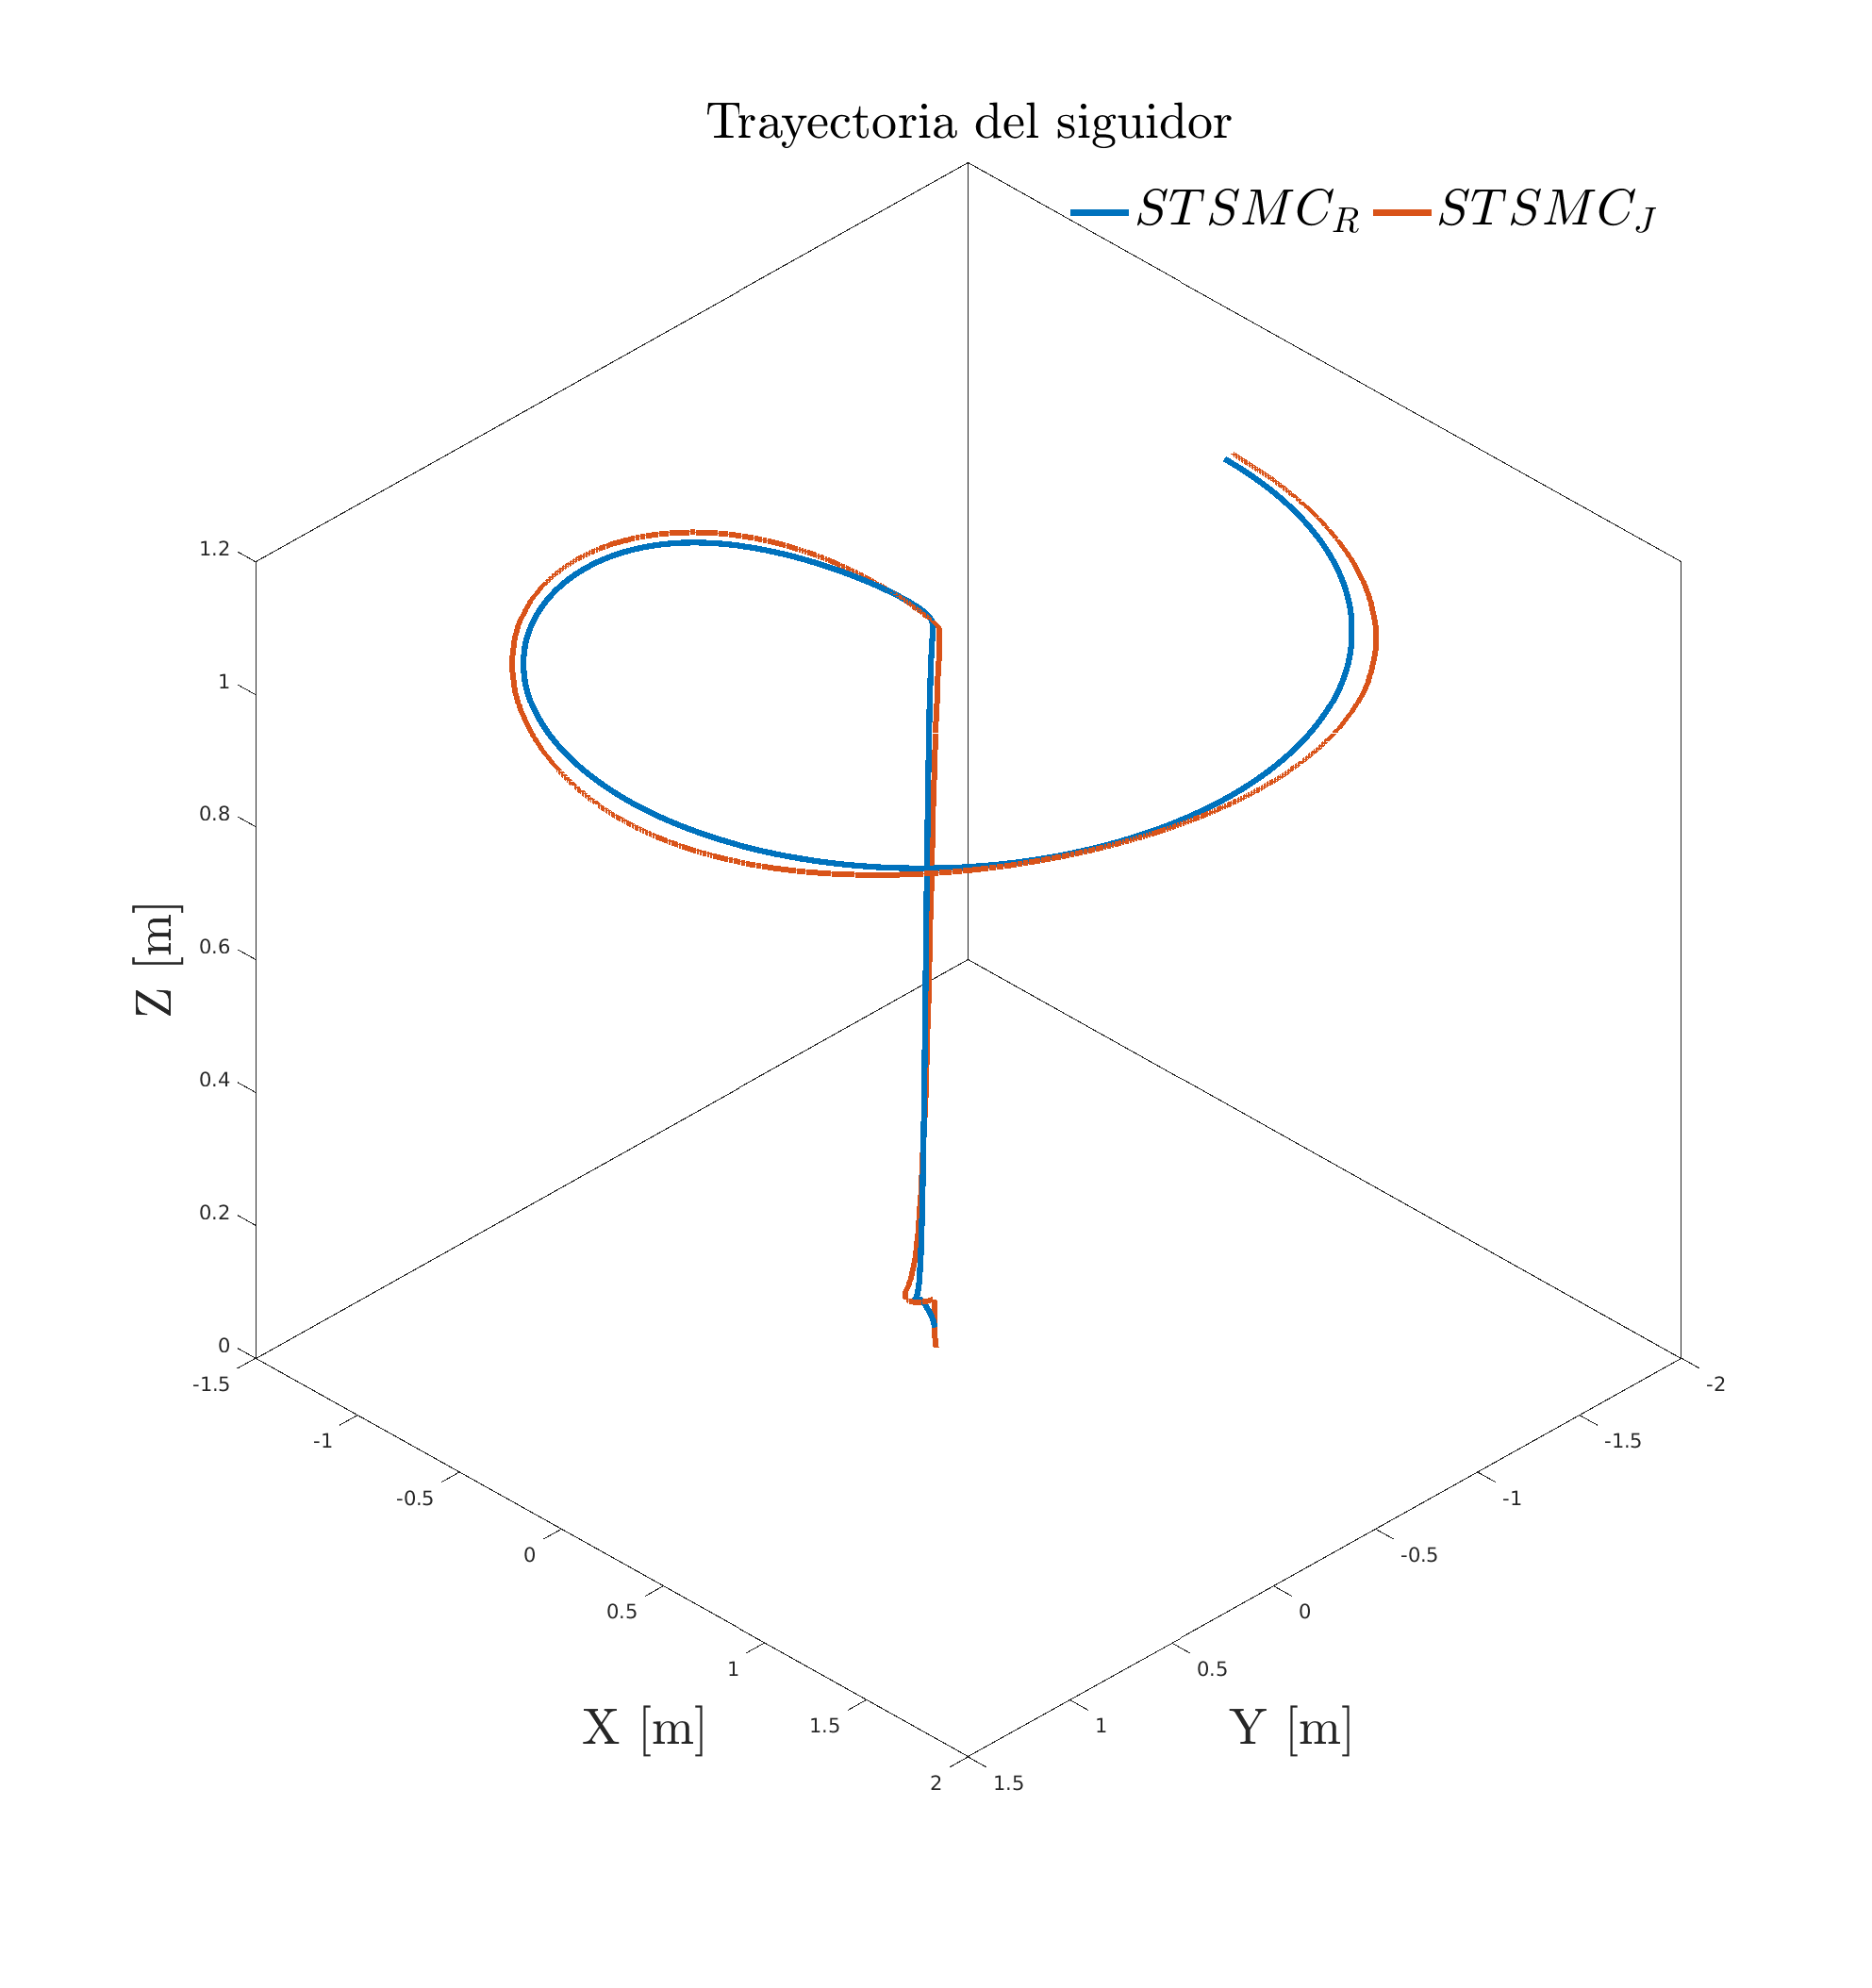
\includegraphics[scale=.18]{Figures/F13.eps}
%\caption{Comparativa de la trayectoria del seguidor}\label{fig:tray seg}
%\end{figure}
%\end{frame}
%
%\begin{frame}{Simulaciones}
%\begin{figure}
%\centering
%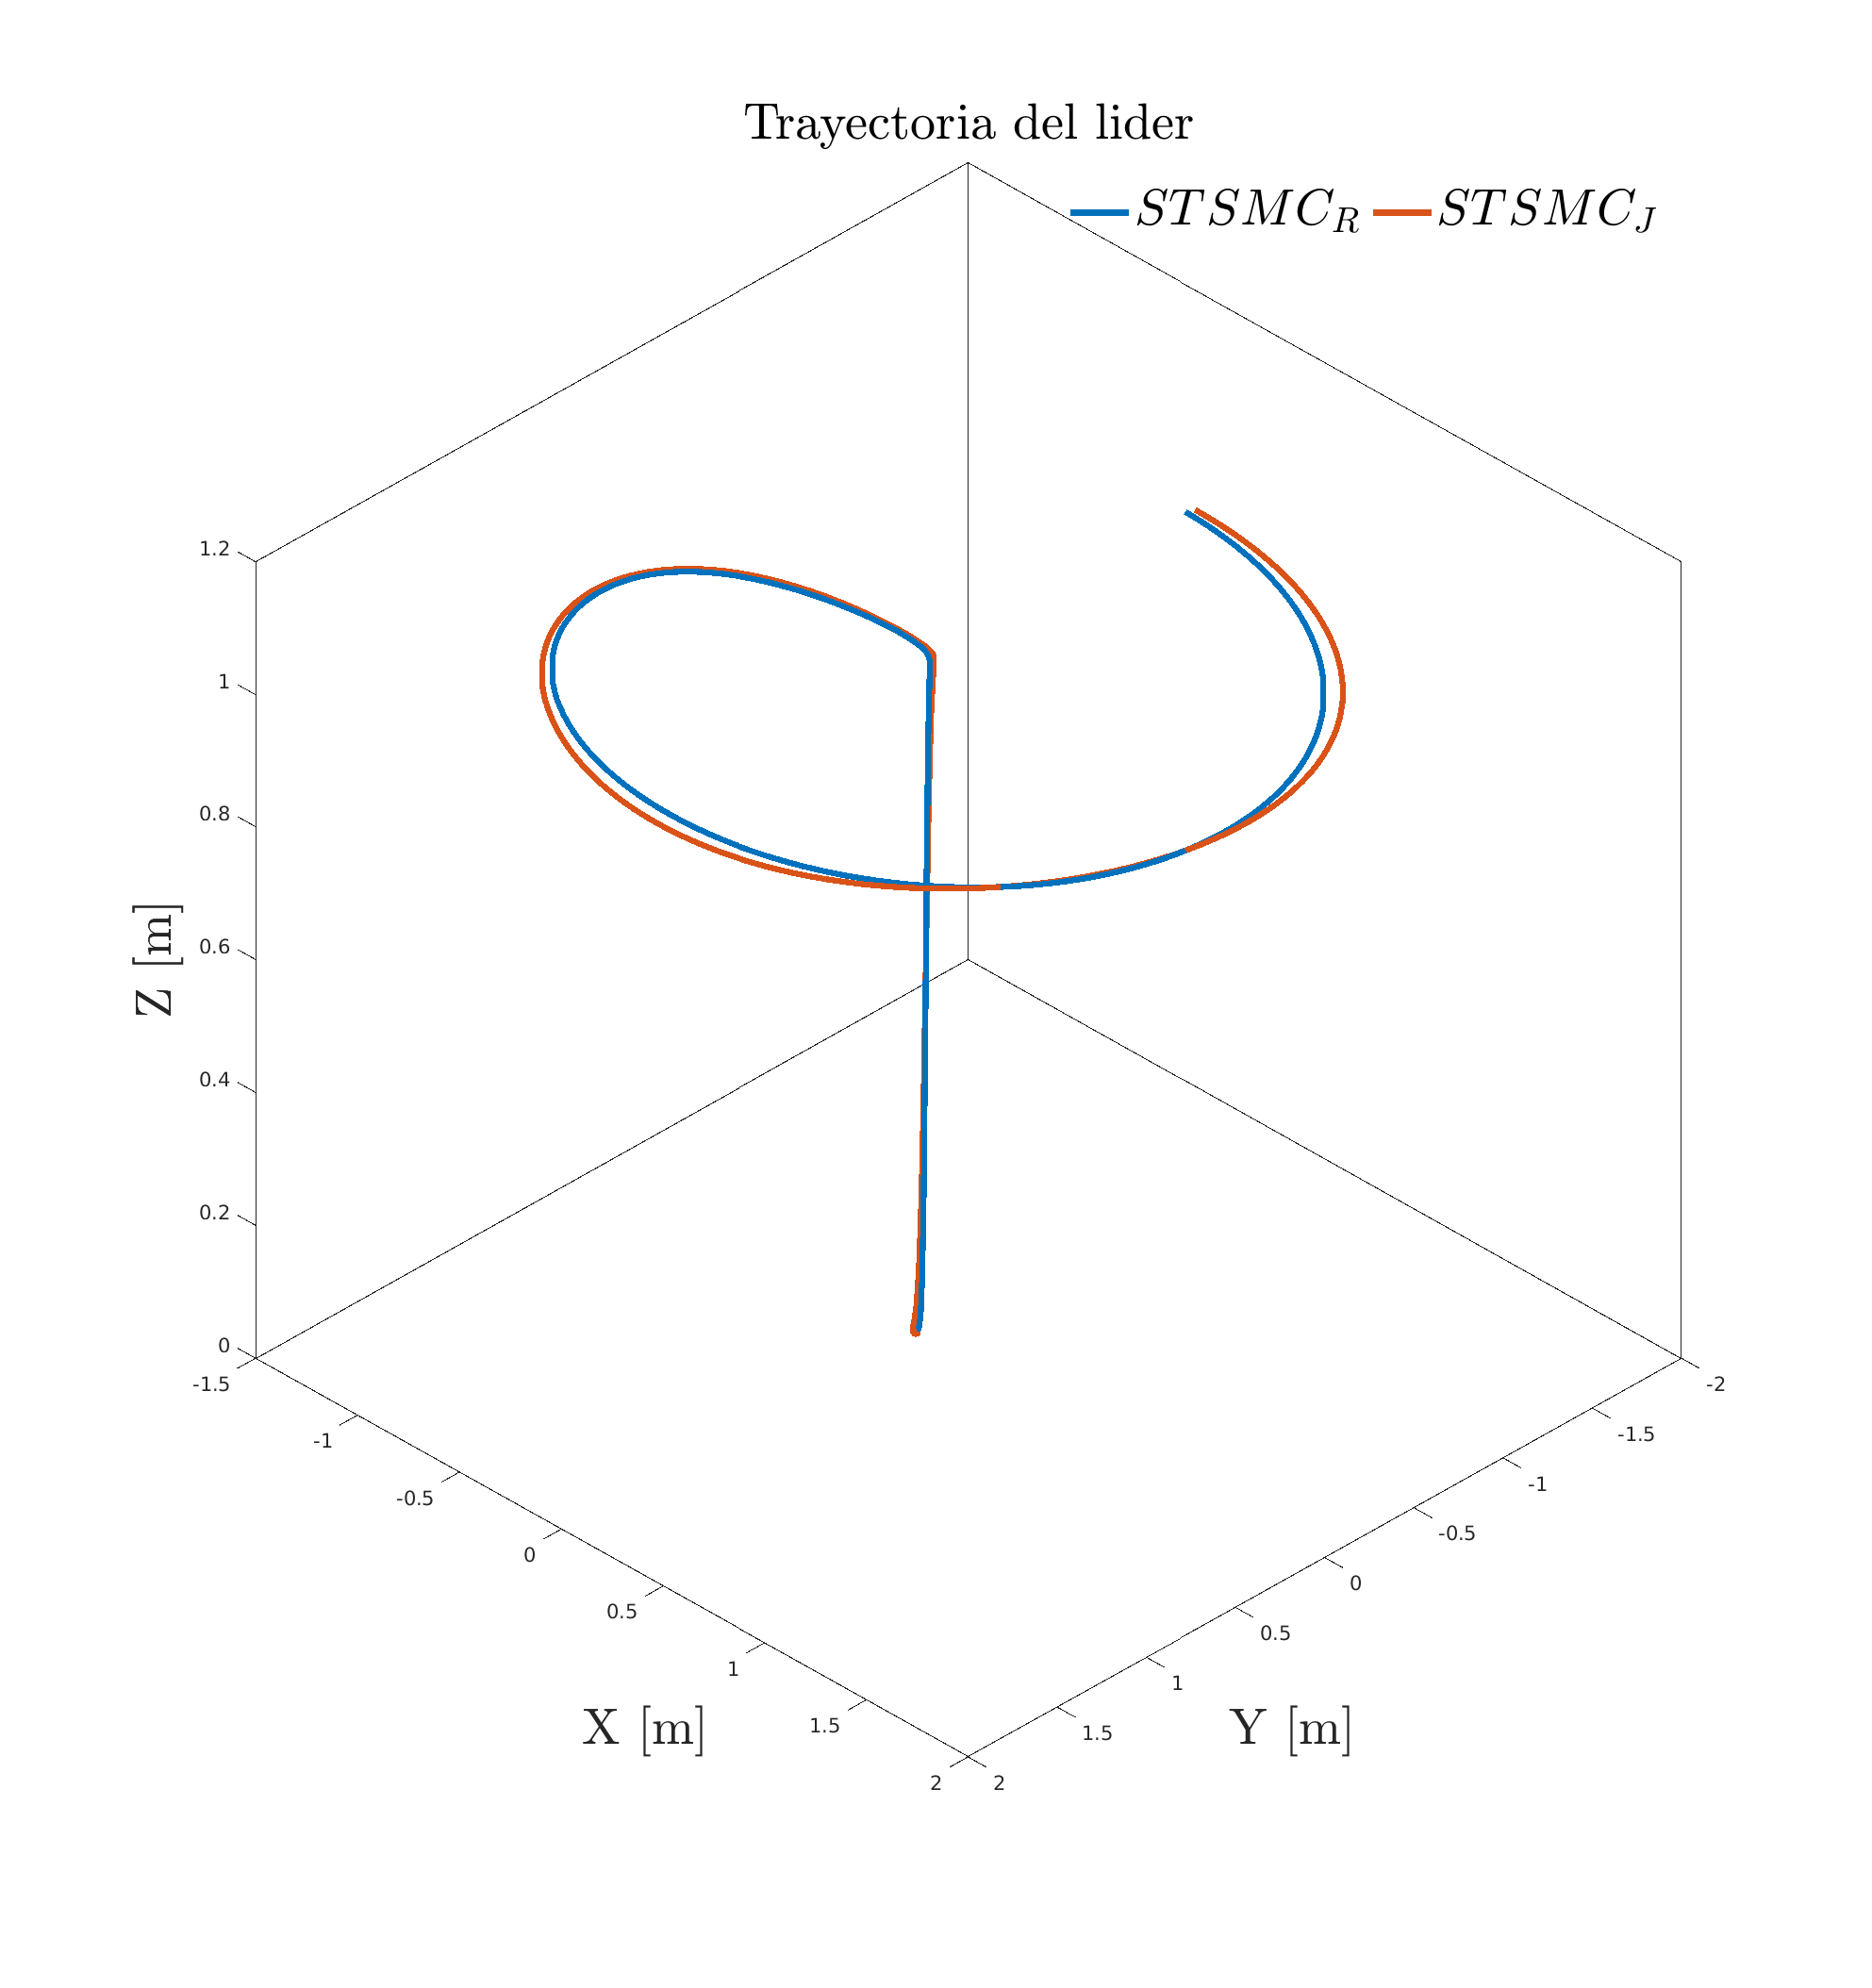
\includegraphics[scale=.18]{Figures/F14.eps}
%\caption{Comparativa de la trayectoria del seguidor}\label{fig:tray lid}
%\end{figure}
%\end{frame}
%
%\begin{frame}{Simulaciones}
%\begin{figure}
%\centering
%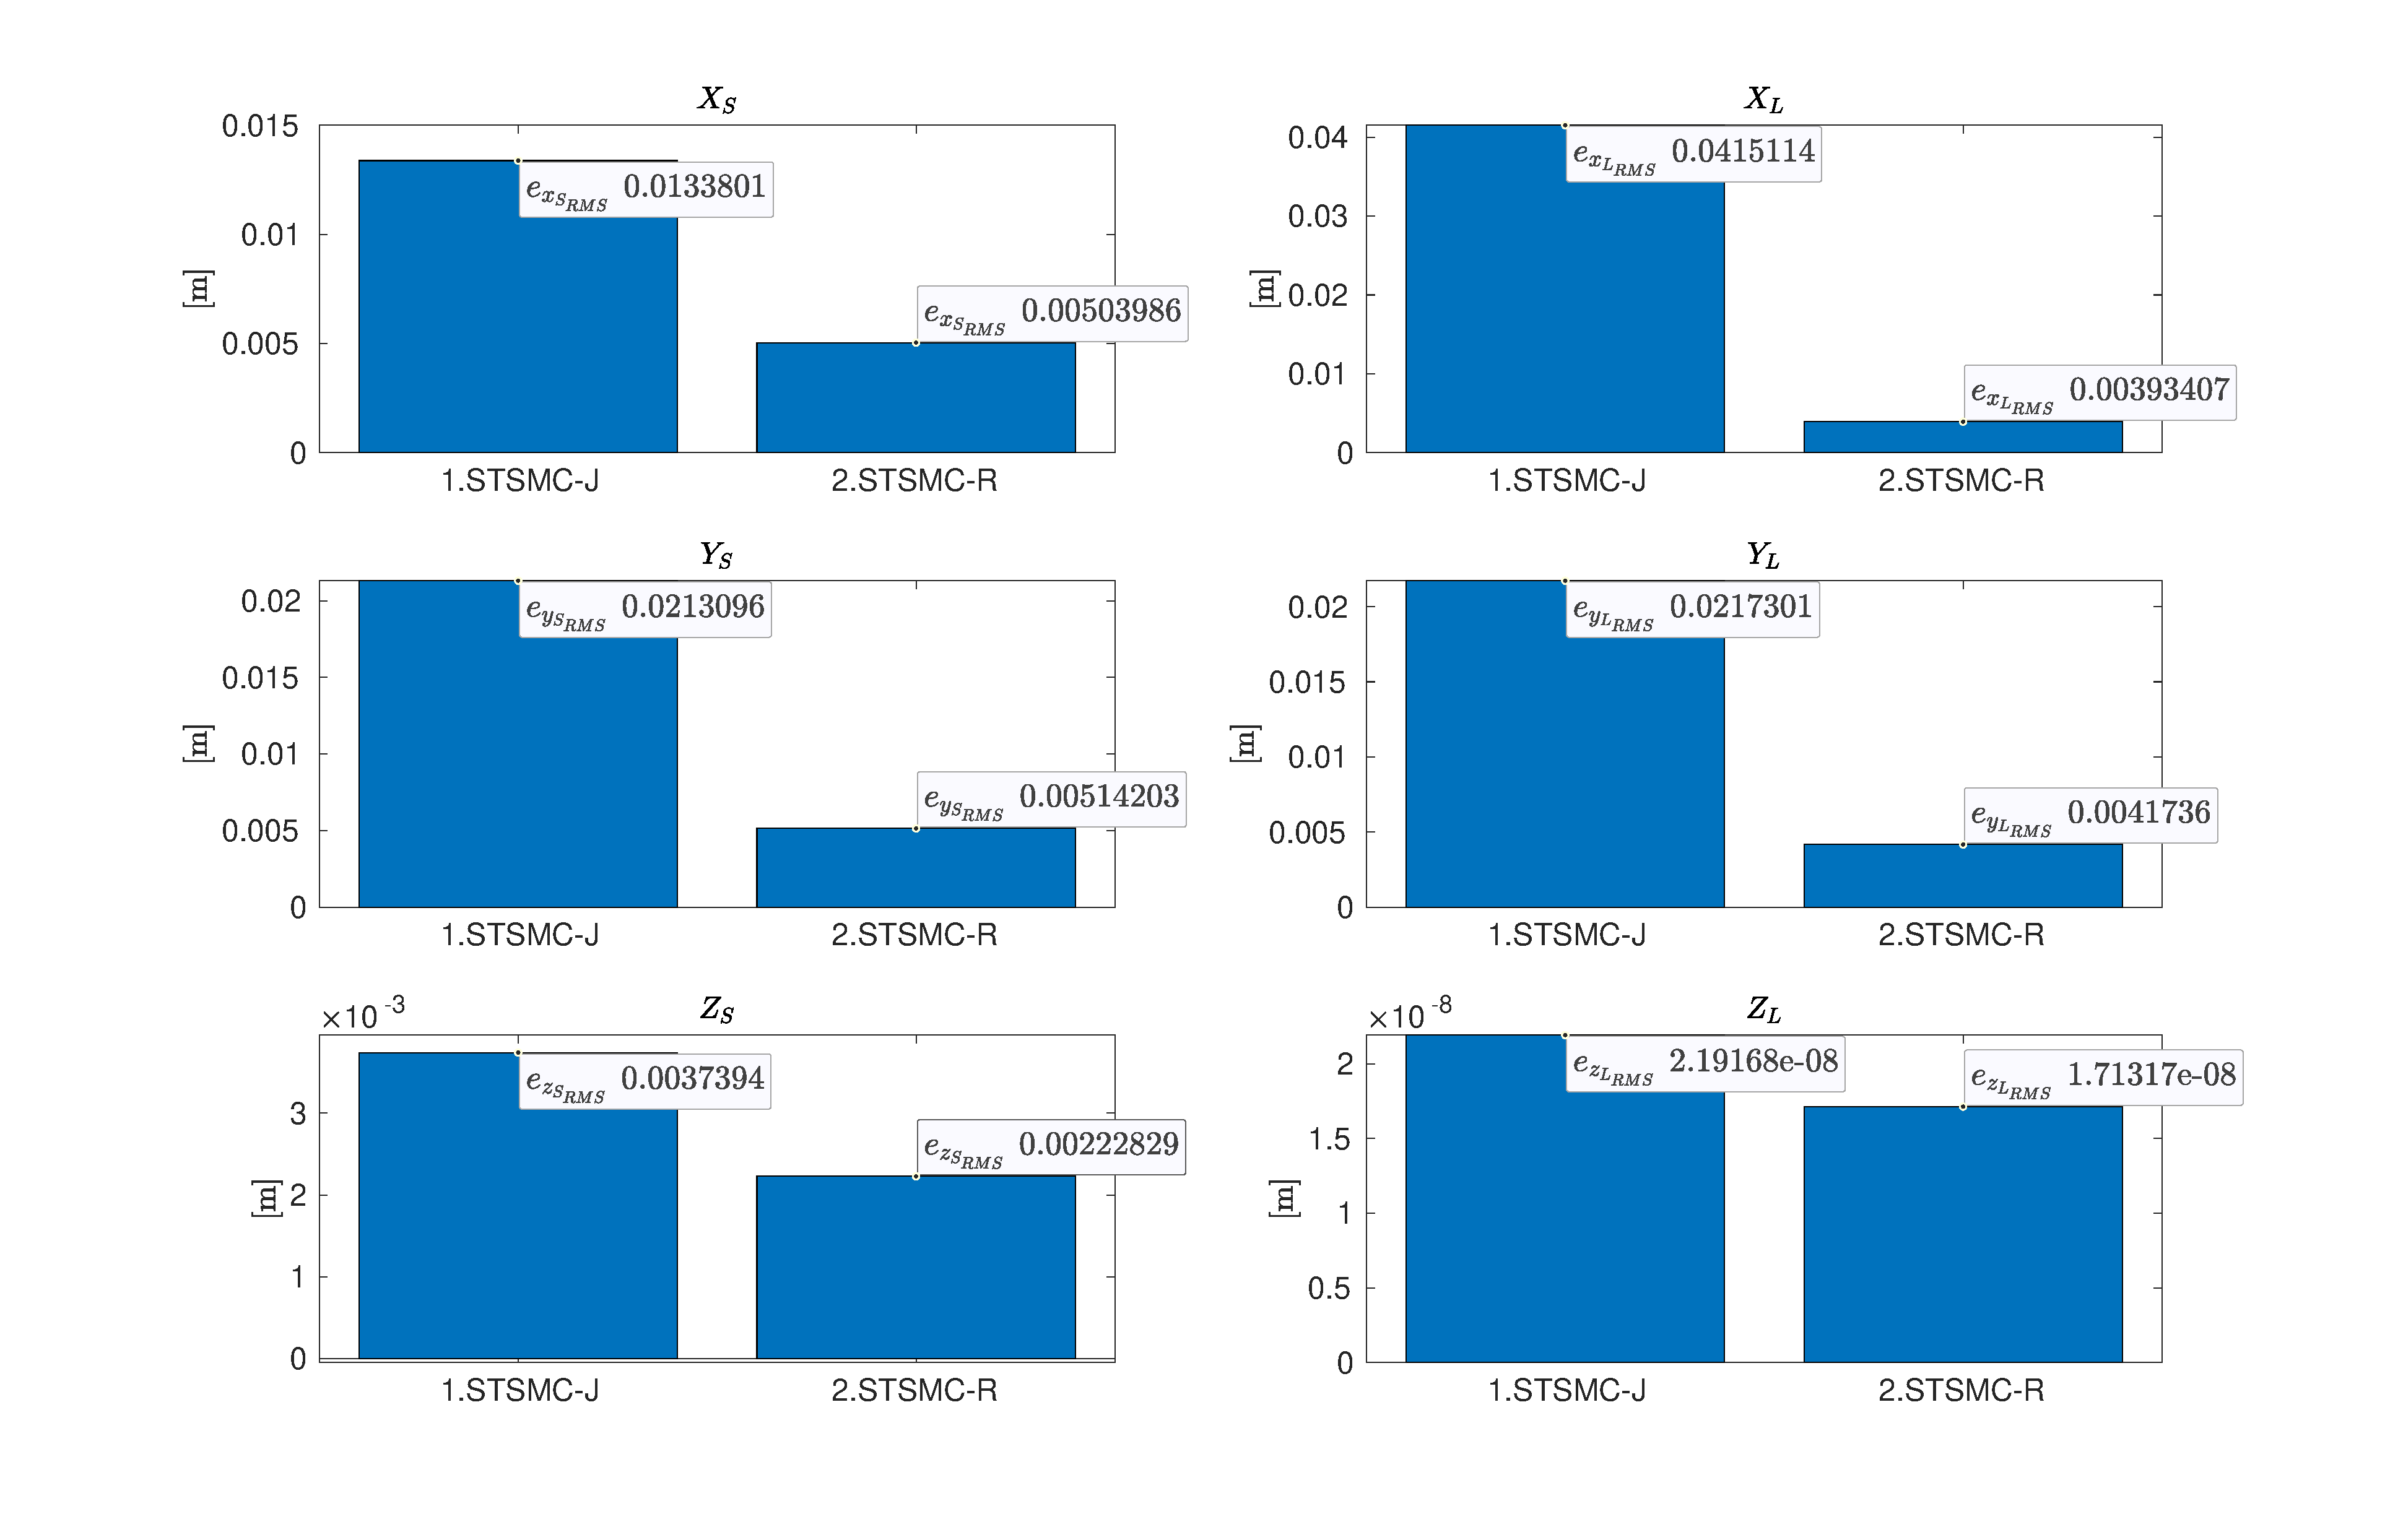
\includegraphics[scale=.17]{Figures/F1.eps}
%\caption{Índices de desempeño de posici\'on.}\label{fig: Indices de desempeno posicion}
%\end{figure}
%\end{frame}
%
%\begin{frame}{Simulaciones}
%\begin{figure}
%\centering
%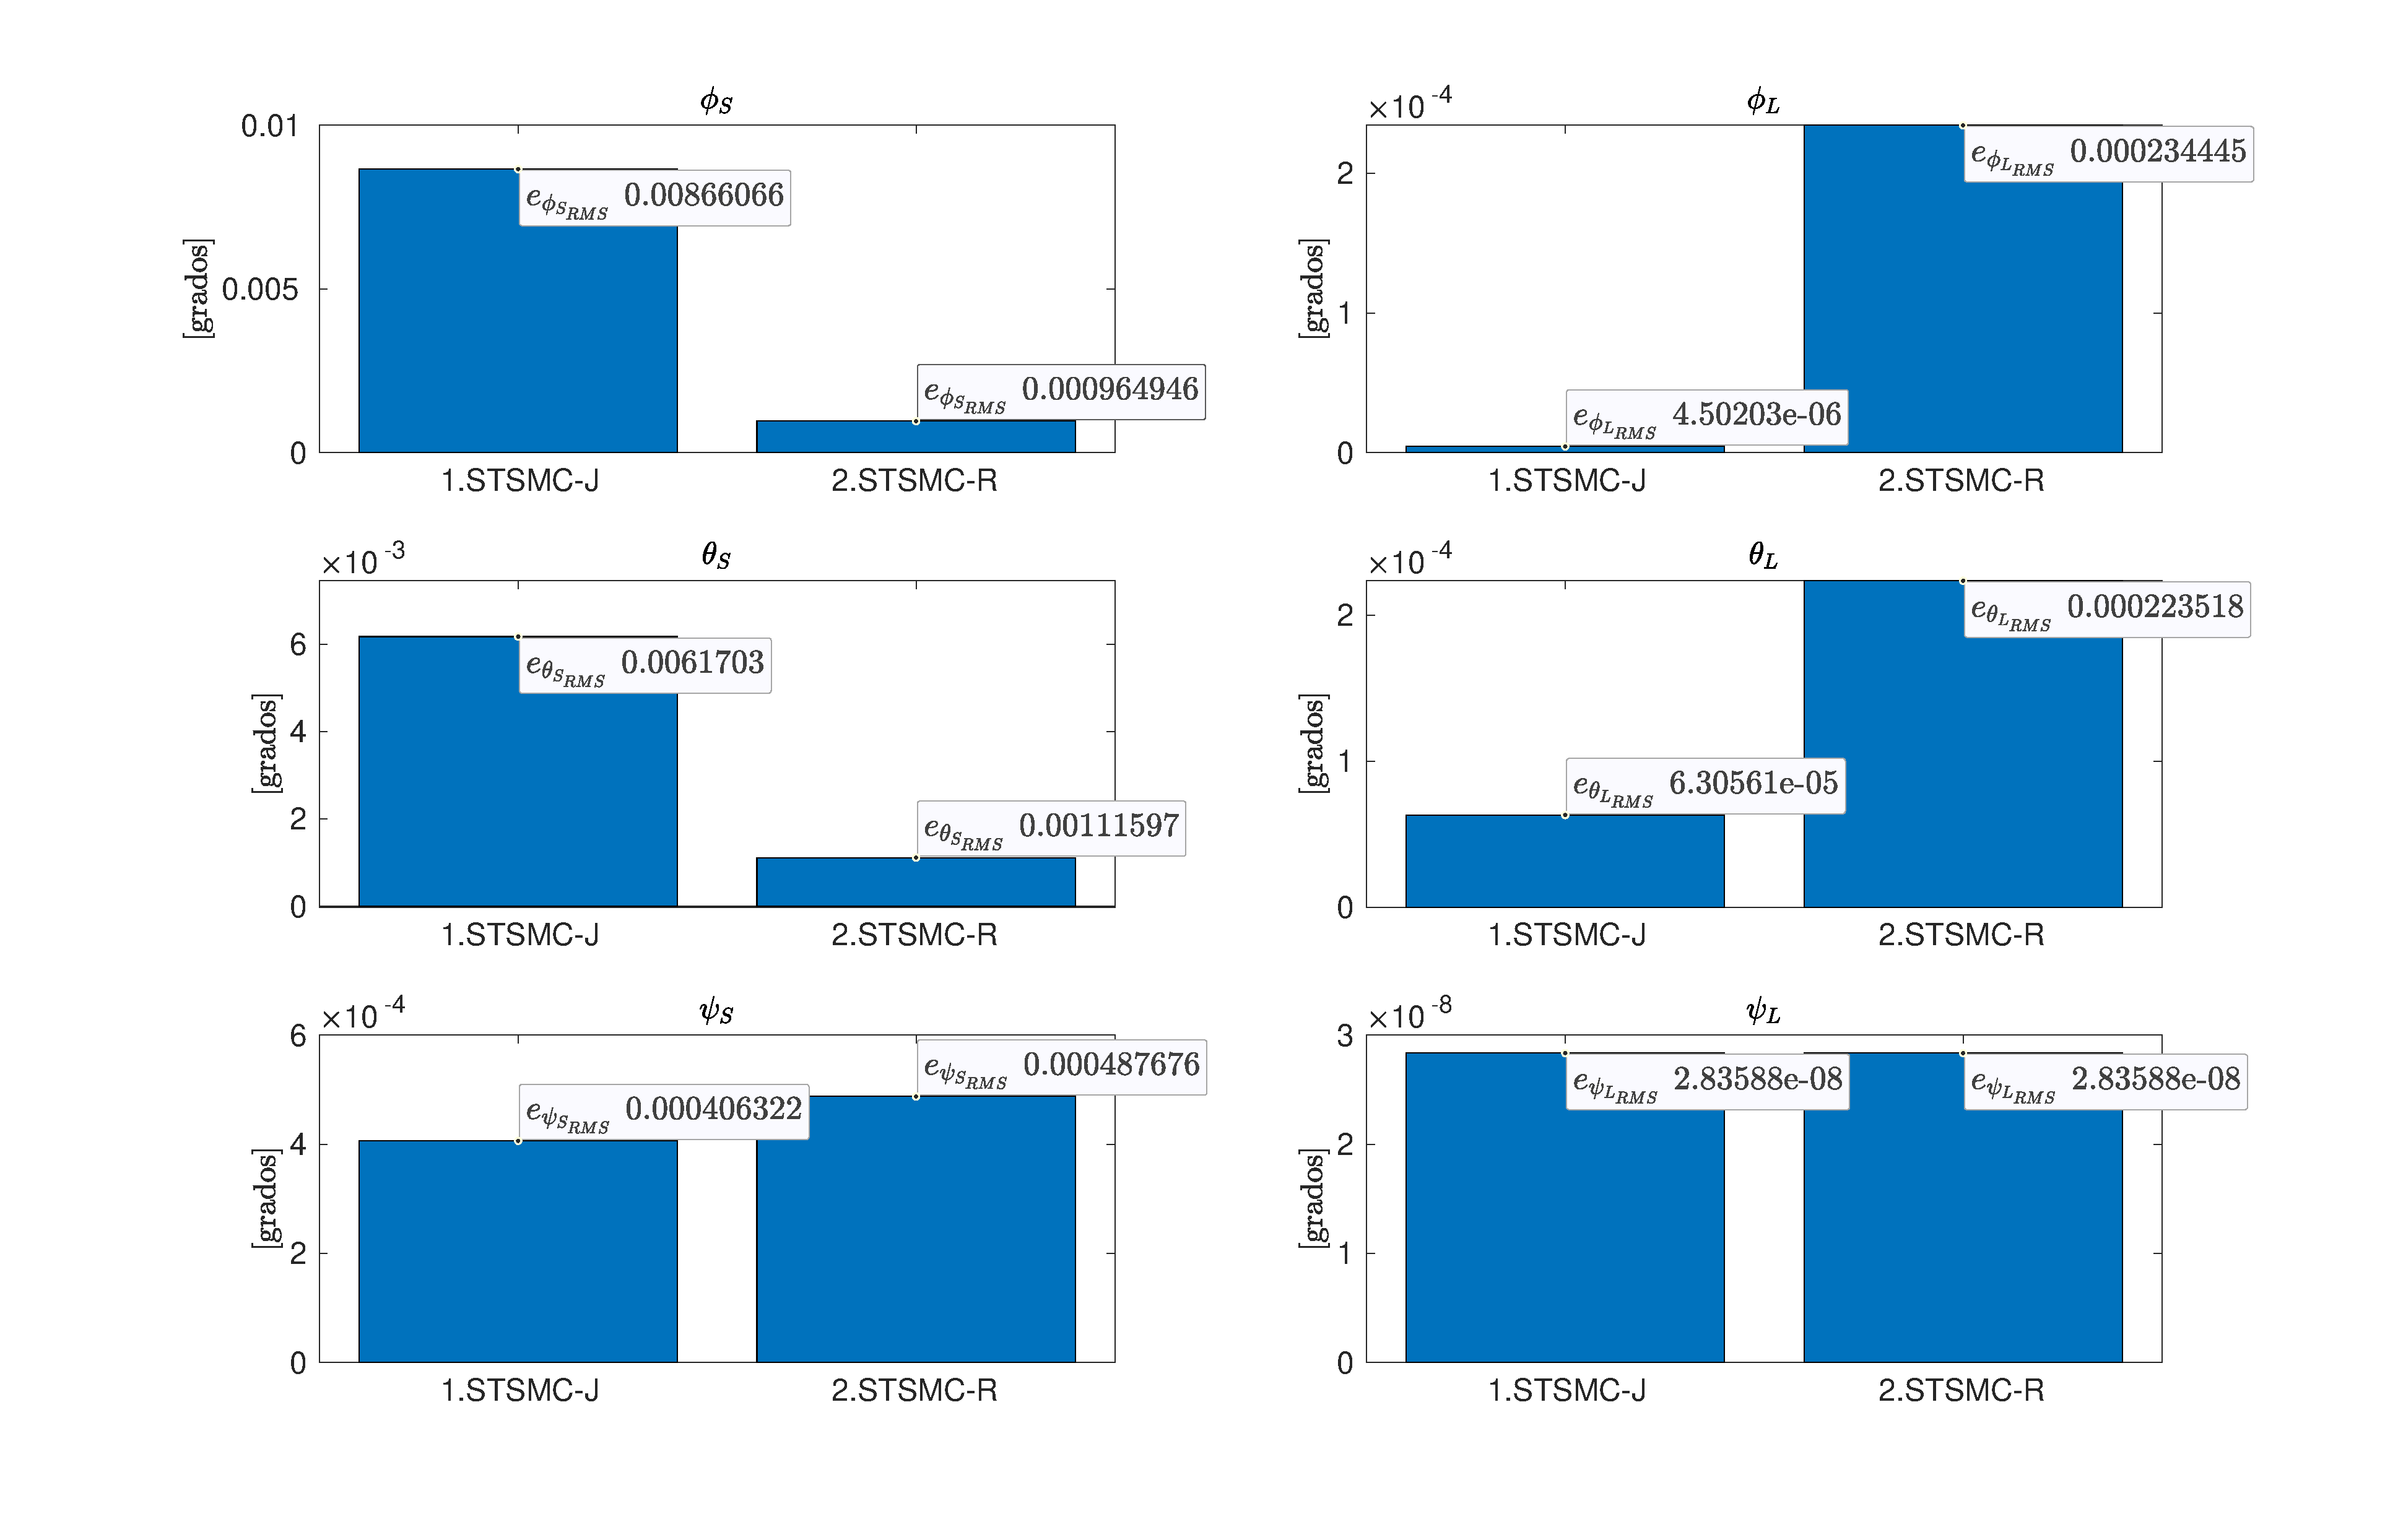
\includegraphics[scale=.17]{Figures/F2.eps}
%\caption{Índices de desempeño de orientaci\'on.}\label{fig: Indices de desempeno orientacion}
%\end{figure}
%\end{frame}
%
%
%\begin{frame}{Simulaciones}
%\begin{figure}
%\centering
%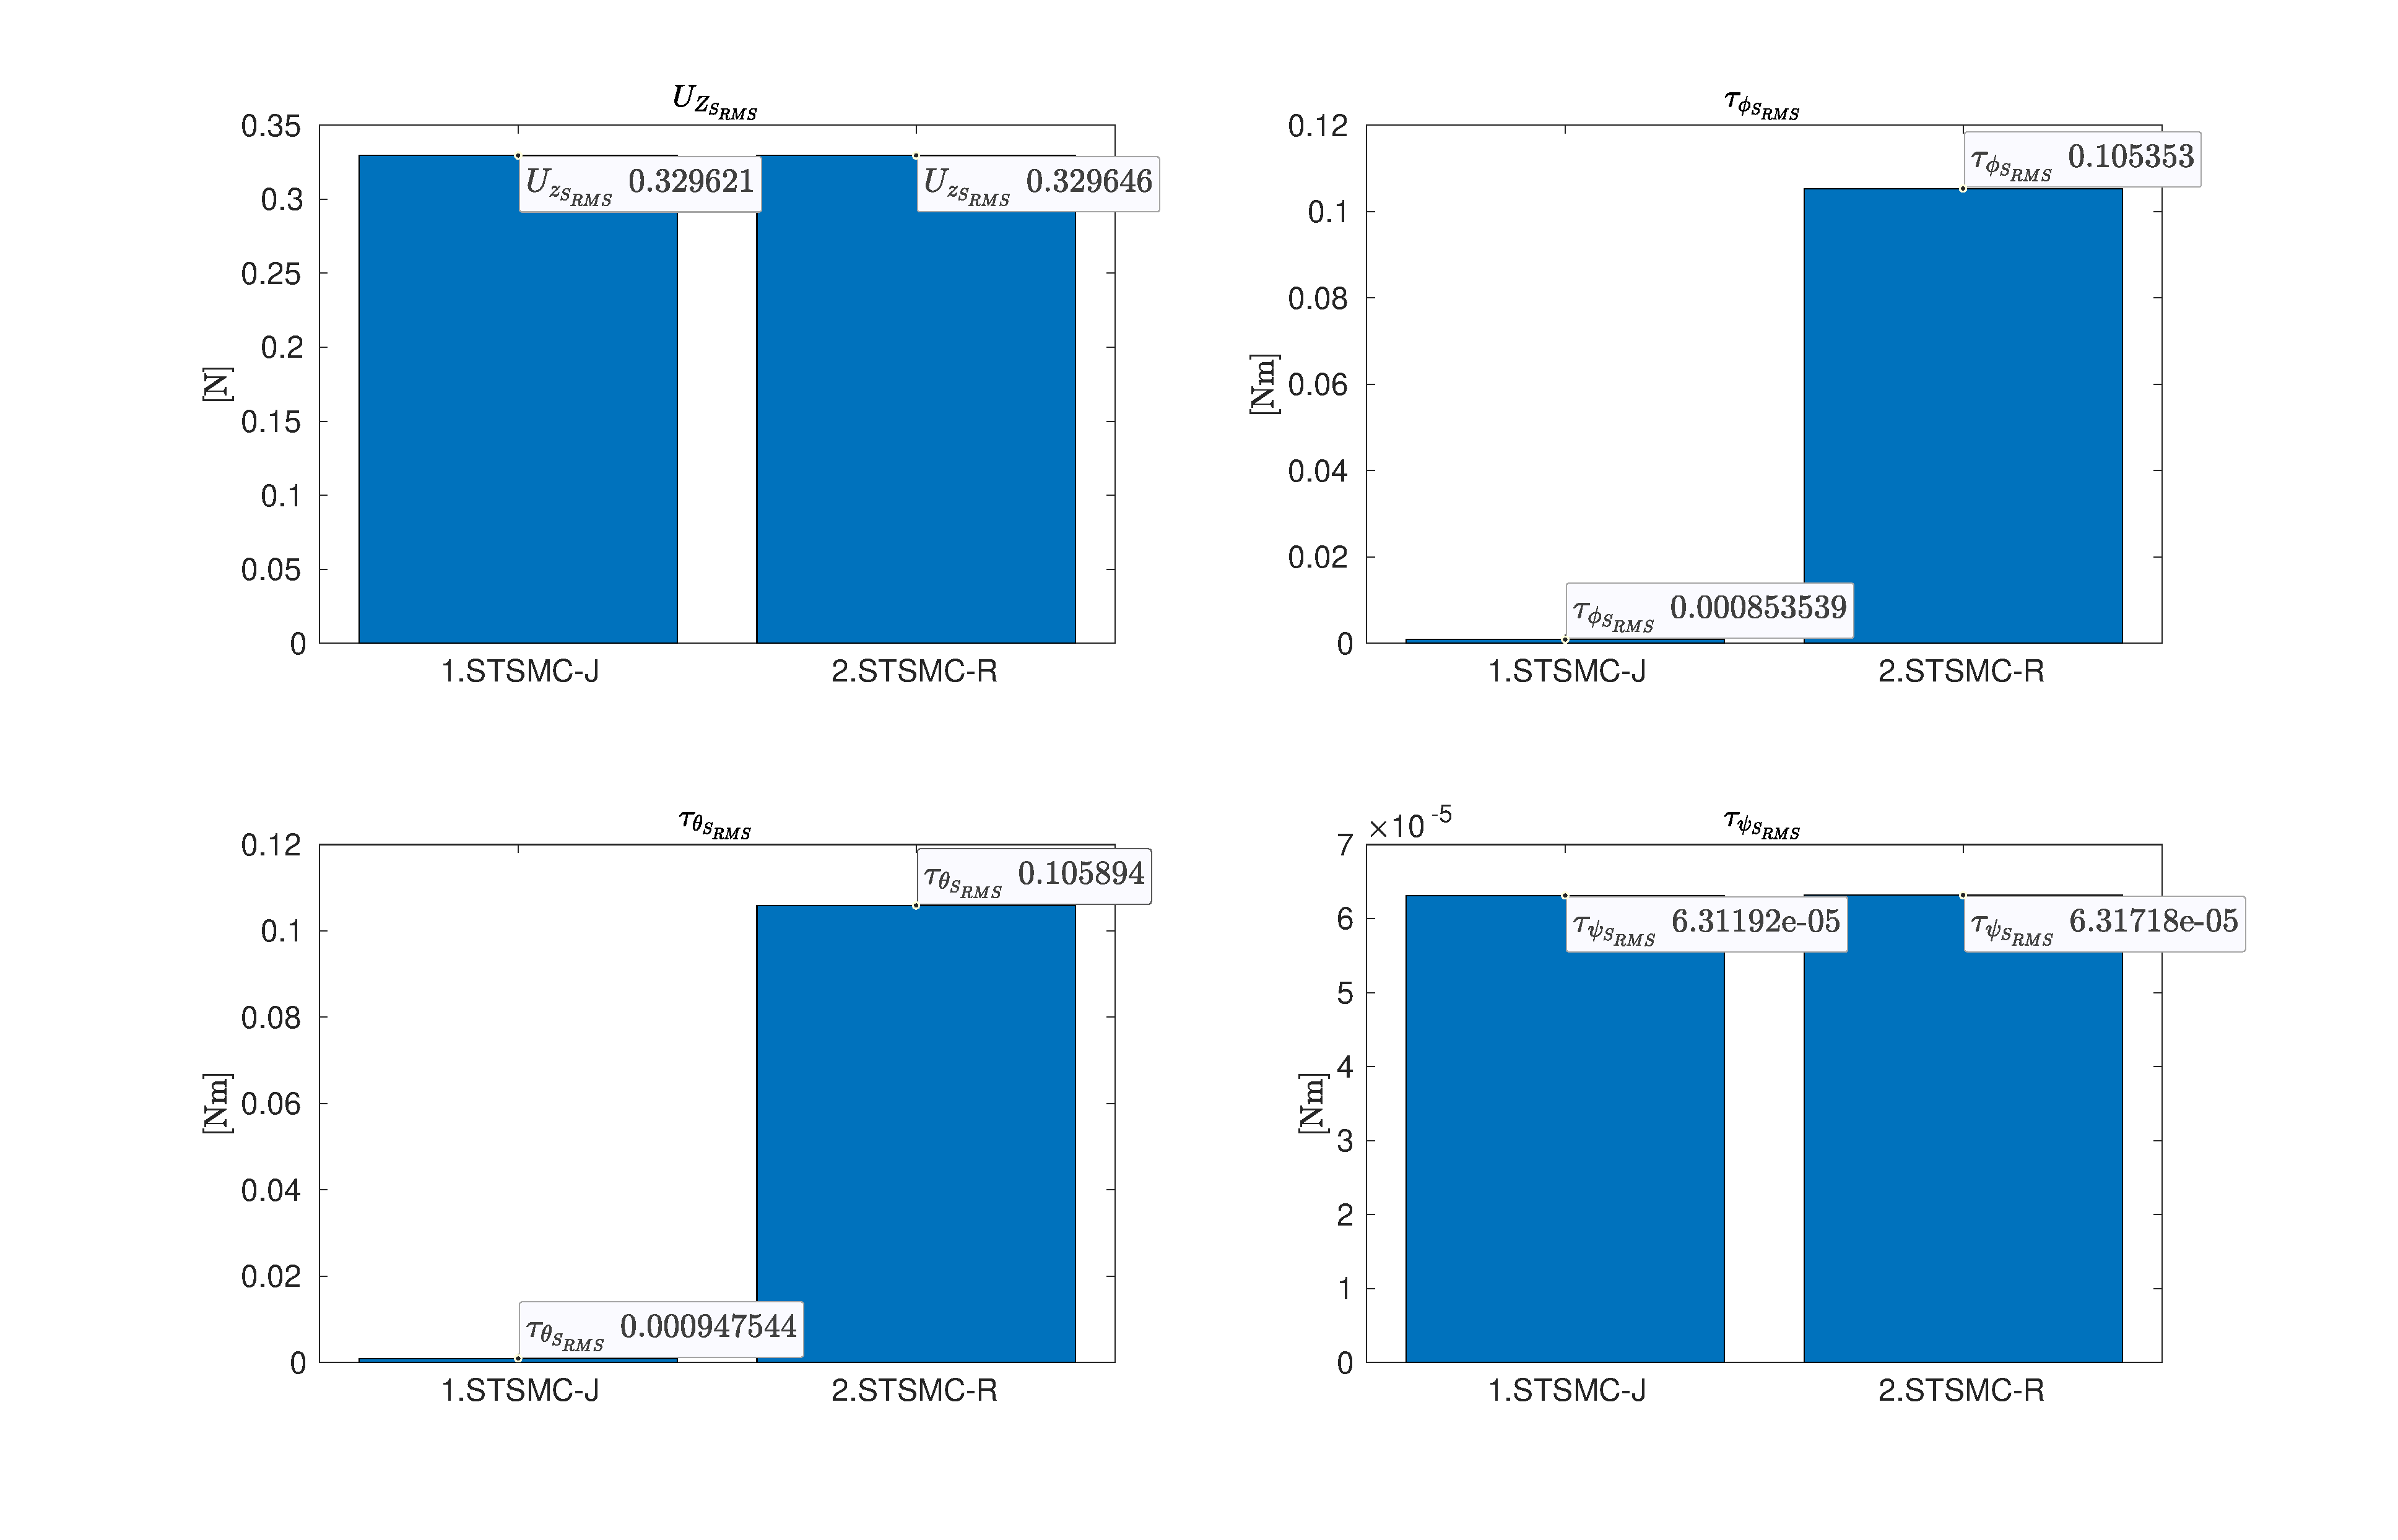
\includegraphics[scale=.17]{Figures/F3.eps}
%\caption{Índices de desempeño de posici\'on.}\label{fig: Indices de desempeno posicion}
%\end{figure}
%\end{frame}
%
%\begin{frame}{Simulaciones}
%\begin{figure}
%\centering
%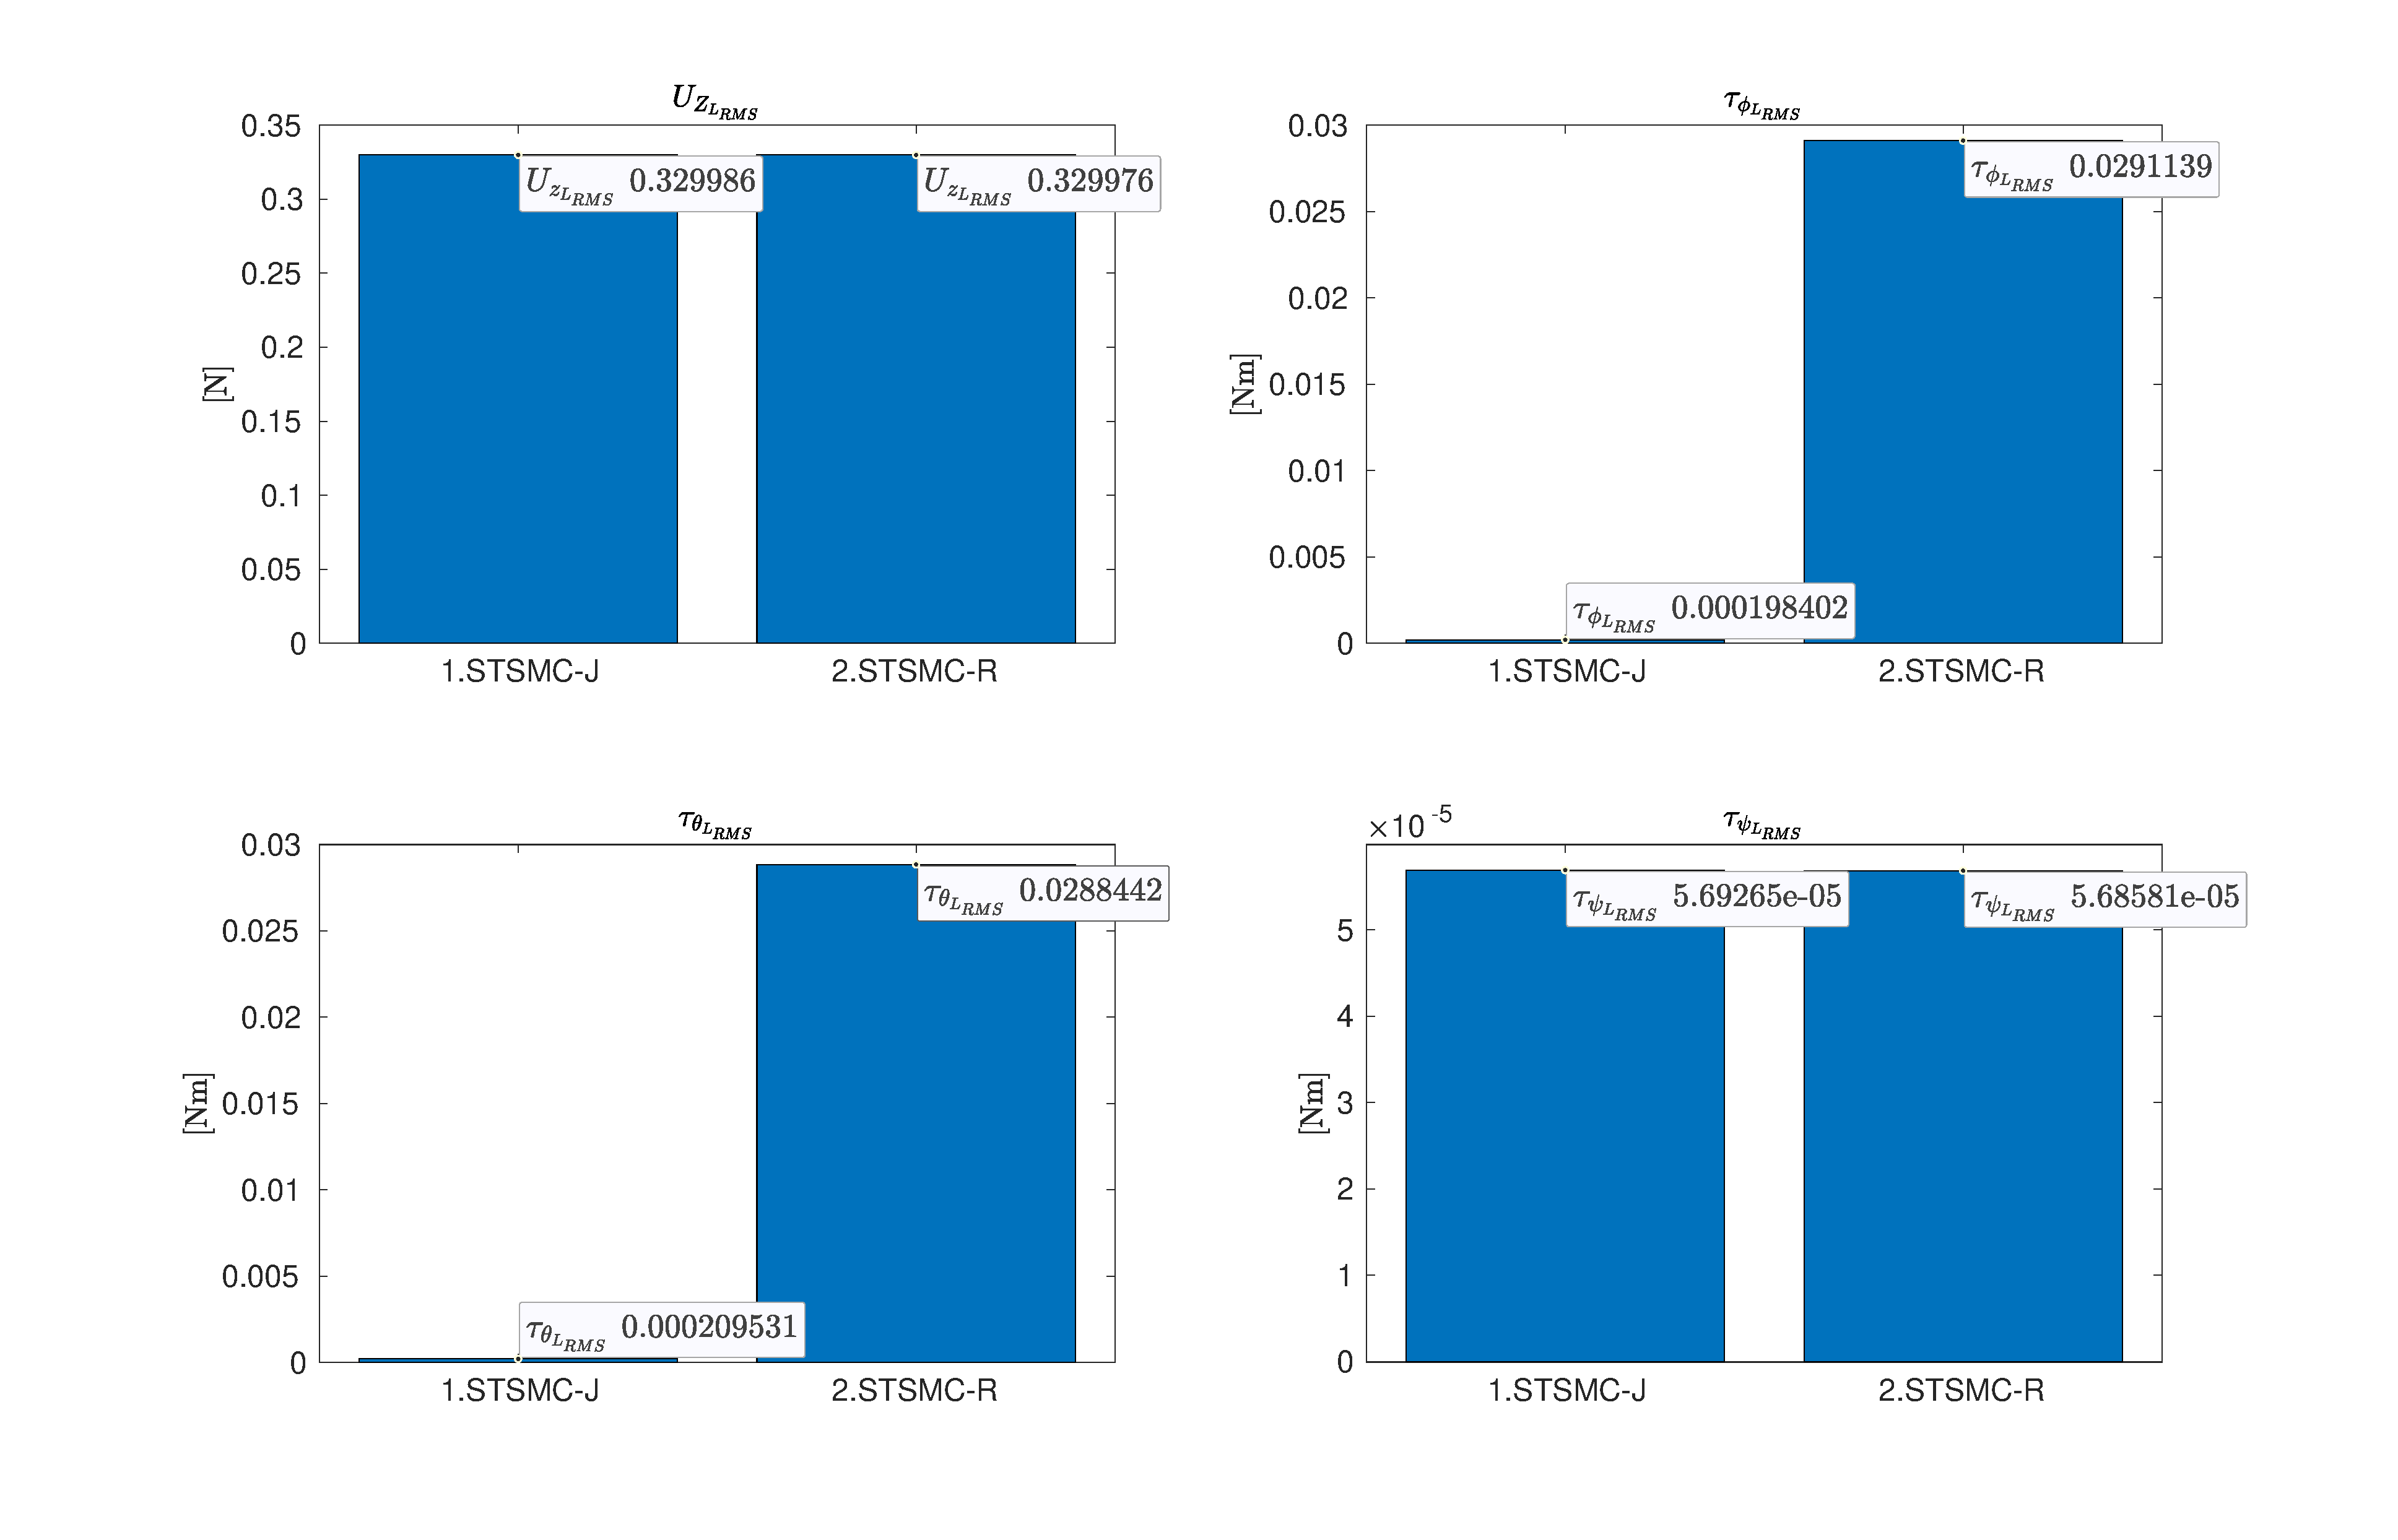
\includegraphics[scale=.17]{Figures/F4.eps}
%\caption{Índices de desempeño de orientaci\'on.}\label{fig: Indices de desempeno orientacion}
%\end{figure}
%\end{frame}

\section{Experimentación.}
\begin{frame}{Experimentación}
\centering
\textbf{¿Como funciona múltiples Crazyflie con ROS? 
}	
\end{frame}


\begin{frame}{Experimentación}
\begin{figure}[h]
	
	\centering  
	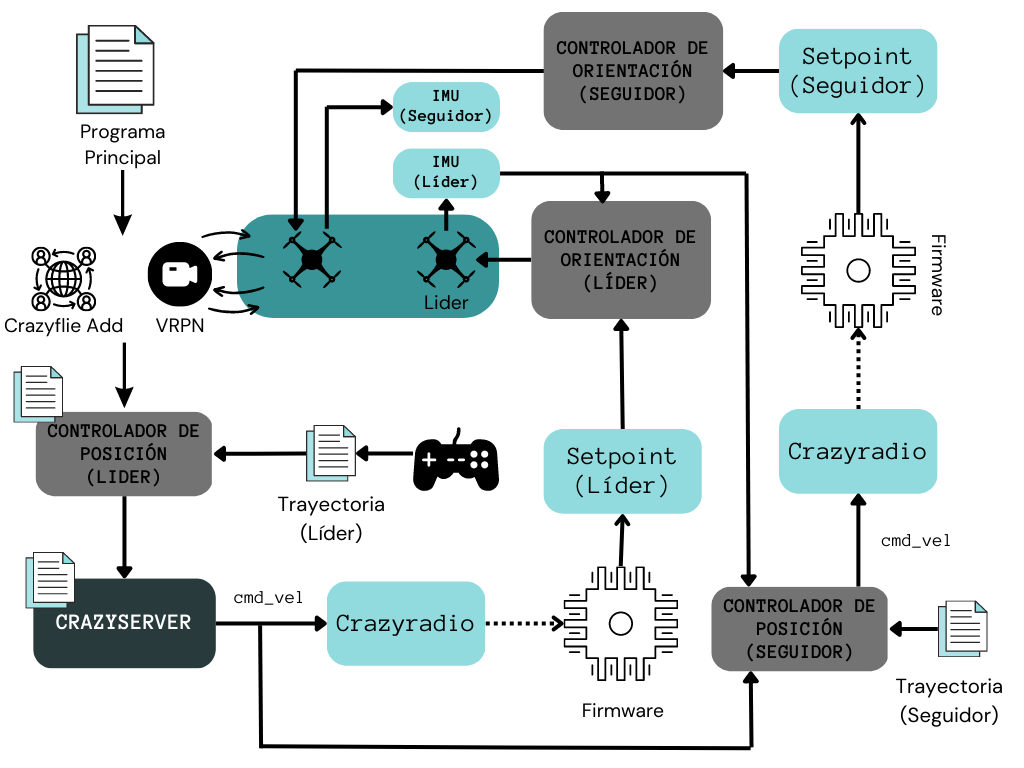
\includegraphics[width=0.85\linewidth]{Figures/Diagrama.png}
	\caption{Diagrama de conexión}\label{Diagrama de conexion}
\end{figure}
\end{frame}


\begin{frame}{Experimentación}
En la versión actual de Motive no es posible modificar los marcos de referencia preestablecidos, que difieren de los utilizados comúnmente. Para solucionar este problema, se ha modificado el código de \textit{vrpn\_client\_ros} de ROS, que proporciona el enlace con la computadora del equipo Quanser, para obtener la posición y orientación requeridas.
\begin{equation*}
	\begin{bmatrix}
		x_{Motive} \\
		y_{Motive} \\
		z_{Motive}
	\end{bmatrix}
	\Rightarrow
	\begin{bmatrix}
		x_{real} \\
		-z_{real} \\
		y_{real}
	\end{bmatrix}	
\end{equation*}
\begin{equation*}
	\begin{bmatrix}
		x_{Motive} \\
		y_{Motive} \\
		z_{Motive}\\
		w_{Motive}
	\end{bmatrix}
	\Rightarrow
	\begin{bmatrix}
		x_{real} \\
		-z_{real} \\
		y_{real}\\
		w_{real}
	\end{bmatrix}
\end{equation*}
\end{frame}



\begin{frame}{Experimentación}
Se han realizado mejoras en el sistema de generación de trayectorias mediante la creación de un nuevo archivo que incluye las coordenadas $x$, $y$, $z$ y $psi$. Esto permite una mayor flexibilidad en las tareas de seguimiento. A diferencia del archivo anterior, que generaba la trayectoria mediante puntos y requería una actualización manual constante en caso de cambios en algún parámetro, el nuevo archivo permite una actualización sin interrupciones y no exige un tiempo de muestreo en cada punto.
\vspace{.5 cm}

Se ha añadido una nueva configuración que permite iniciar la trayectoria al presionar el botón 5 del joystick y reiniciarla al presionar el mismo botón. Esto mejora el control en la ejecución de las demostraciones y proporciona una experiencia más intuitiva al usuario.
\end{frame}

\begin{frame}{Experimentación}
Se han creado dos nuevos archivos para los controladores de posición del líder y el seguidor, utilizando la metodología presentada previamente. Gracias a esta mejora, se ha logrado una mejoría significativa en el seguimiento de un Quad-Rotor en comparación con el controlador previo. Actualmente, se está trabajando en la metodología Líder-Seguidor con el objetivo de validar su funcionamiento con controladores multi-agentes.
\begin{figure}[h]
	\centering  
	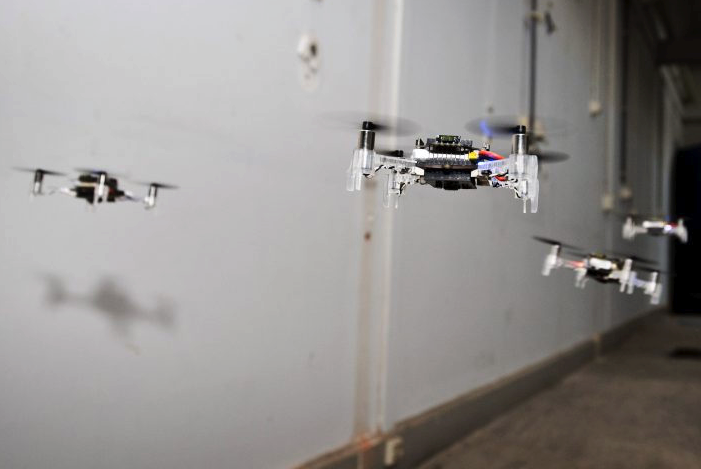
\includegraphics[width=0.4\linewidth]{Figures/CFSwarm.png}
\end{figure}
\end{frame}

\begin{frame}{Banco de pruebas y Firmware}
Se ha diseñado un banco de pruebas para sintonizar los controladores propuestos, tambien se realizo el dise\~no de una base para los marcadores y una base para los motores. Además, se ha agregado el código de los controladores SMC, Backstepping, STA, TC, STSMC, NTSMC y PID, los cuales generan señales de control en newtons y newton metro. También se han agregado funciones adicionales al firmware, como la función de signo y la función para convertir las señales de control de newton a RPM, ya que el sistema requiere las señales de control en RPM para su correcto funcionamiento.
	\begin{figure}[h]
		\centering  
		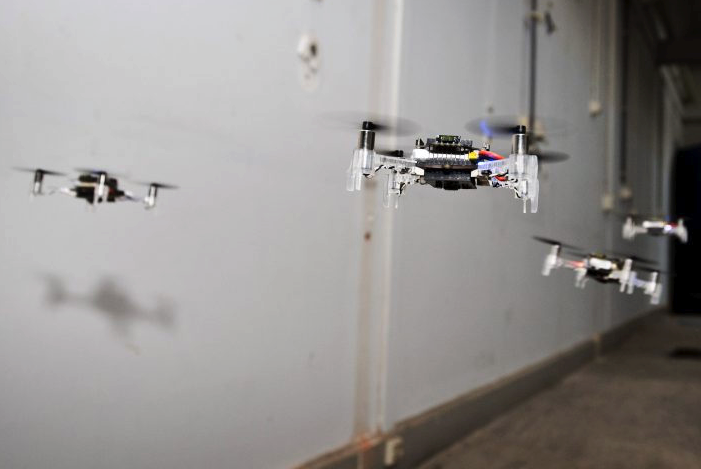
\includegraphics[width=0.4\linewidth]{Figures/CFSwarm.png}
	\end{figure}
\end{frame}


\begin{frame}{Github}
Se ha desarrollado un programa en MATLAB y ROS para graficar las señales de interés generadas por el Quad-Rotor y sus controladores. Además, se han creado dos repositorios que contienen los archivos mencionados anteriormente, permitiendo un fácil acceso y descarga de los mismos para su uso y mejora continua.

Estas mejoras permiten una mayor visualización y análisis de las señales generadas, lo que facilita la identificación y solución de posibles errores en el sistema de control. Además, la disponibilidad de los repositorios en Github, permite tener un mejor control de versiones, y un respaldo de los archivos.
\end{frame}


\section{Conclusiones}
\begin{frame}{Conclusiones}
Este trabajo presenta:
\begin{itemize}
    \item Una comparativa de las técnicas para el c\'alculo de las referencias deseadas entre \footfullcite{rios2018continuous} y \footfullcite{inproceedings}.

    \item Se utiliza el controlador STSMC (Singular Terminal Sliding Mode Control) utilizando el esquema líder- seguidor en simulación, actualmente se tienen los controladores SMC, Backstepping, STA, TC, NTSMC y PID, en simulaci\'on

    \item La técnica utilizada para las se\~nales de control del sistema no linealizado muestra un mejor desempe\~no, que las otras propuestas, ya que contempla todos los estados.
    

\end{itemize}


\end{frame}

\section{Conclusiones}
\begin{frame}{Conclusiones}
	Este trabajo presenta:
	\begin{itemize}
    \item Se sintonizo el controlador de posición propuesto, para el líder, y actualmente se esta trabajando el seguidor.

	\item Se sintonizaron los controladores de orientación, Backstepping, SMC, STA, NTSMC, y se probaron con los sensores Multiranger Deck y Flow Deck
	
	\item Se desarrollo el dise\~no de un banco de pruebas.
	
	\item Se generaron dos repositorios, uno para el firmware modificado y otro para el espacio de trabajo de ROS.
	\end{itemize}
	
	
\end{frame}






\end{document}

